%definira klasu dokumenta 
\documentclass[12pt]{report} 

%prostor izmedu naredbi \documentclass i \begin{document} se zove uvod. U njemu se nalaze naredbe koje se odnose na cijeli dokument
	
	%osnovni LaTex ne može riješiti sve probleme, pa se koriste različiti paketi koji olakšavaju izradu željenog dokumenta
	\usepackage[croatian]{babel} 
	\usepackage{amssymb}
	\usepackage{amsmath}
	\usepackage{txfonts}
	\usepackage{mathdots}
	\usepackage{titlesec}
	\usepackage{array}
	\usepackage{lastpage}
	\usepackage{etoolbox}
	\usepackage{tabularray}
	\usepackage{color, colortbl}
	\usepackage{adjustbox}
	\usepackage{geometry}
	\usepackage[classicReIm]{kpfonts}
	\usepackage{hyperref}
	\usepackage{fancyhdr}
	
	\usepackage{float}
	\usepackage{setspace}
	\restylefloat{table}
	
	
	\patchcmd{\chapter}{\thispagestyle{plain}}{\thispagestyle{fancy}}{}{} %redefiniranje stila stranice u paketu fancyhdr
	
	%oblik naslova poglavlja
	\titleformat{\chapter}{\normalfont\huge\bfseries}{\thechapter.}{20pt}{\Huge}
	\titlespacing{\chapter}{0pt}{0pt}{40pt}
	
	
	\linespread{1.3} %razmak između redaka
	
	\geometry{a4paper, left=1in, top=1in, right=1in}  %oblik stranice
	
	\hypersetup{ colorlinks, citecolor=black, filecolor=black, linkcolor=black,	urlcolor=black }   %izgled poveznice
	
	
	%prored smanjen između redaka u nabrajanjima i popisima
	\newenvironment{packed_enum}{
		\begin{enumerate}
			\setlength{\itemsep}{0pt}
			\setlength{\parskip}{0pt}
			\setlength{\parsep}{0pt}
		}{\end{enumerate}}
	
	\newenvironment{packed_item}{
		\begin{itemize}
			\setlength{\itemsep}{0pt}
			\setlength{\parskip}{0pt}
			\setlength{\parsep}{0pt}
		}{\end{itemize}}
	
	
	
	
	%boja za privatni i udaljeni kljuc u tablicama
	\definecolor{LightBlue}{rgb}{0.9,0.9,1}
	\definecolor{LightGreen}{rgb}{0.9,1,0.9}
	
	%Promjena teksta za dugačke tablice
	\DefTblrTemplate{contfoot-text}{normal}{Nastavljeno na idućoj stranici}
	\SetTblrTemplate{contfoot-text}{normal}
	\DefTblrTemplate{conthead-text}{normal}{(Nastavljeno)}
	\SetTblrTemplate{conthead-text}{normal}
	\DefTblrTemplate{middlehead,lasthead}{normal}{Nastavljeno od prethodne stranice}
	\SetTblrTemplate{middlehead,lasthead}{normal}
	
	%podesavanje zaglavlja i podnožja
	
	\pagestyle{fancy}
	\lhead{Programsko inženjerstvo}
	\rhead{Digitalizacija}
	\lfoot{Kompletići}
	\cfoot{stranica \thepage/\pageref{LastPage}}
	\rfoot{\today}
	\renewcommand{\headrulewidth}{0.2pt}
	\renewcommand{\footrulewidth}{0.2pt}
	
	
	\begin{document} 
		
		
		
		\begin{titlepage}
			\begin{center}
				\vspace*{\stretch{1.0}} %u kombinaciji s ostalim \vspace naredbama definira razmak između redaka teksta
				\LARGE Programsko inženjerstvo\\
				\large Ak. god. 2023./2024.\\
				
				\vspace*{\stretch{3.0}}
				
				\huge Digitalizacija\\
				\Large Dokumentacija, Rev. \textit{2}\\
				
				\vspace*{\stretch{12.0}}
				\normalsize
				Grupa: \textit{Kompletići}\\
				Voditelj: \textit{Martin Ante Rogošić}\\
				
				
				\vspace*{\stretch{1.0}}
				Datum predaje: \textit{19. 1. 2024.}\\
				
				\vspace*{\stretch{4.0}}
				
				Nastavnik: \textit{Igor Stančin}\\
				
			\end{center}
			
			
		\end{titlepage}
		
		
		\tableofcontents
		
		
		\chapter{Dnevnik promjena dokumentacije}
		
		\textbf{\textit{Kontinuirano osvježavanje}}\\
				
		
		\begin{longtblr}[
				label=none
			]{
				width = \textwidth, 
				colspec={|X[2]|X[13]|X[3]|X[3]|}, 
				rowhead = 1
			}
			\hline
			\textbf{Rev.}	& \textbf{Opis promjene/dodatka} & \textbf{Autori} & \textbf{Datum}\\[3pt] \hline
			
			0.1 & Napravljen predložak.	& Martin Ante Rogošić & 7.11.2023. 		\\[3pt] \hline 
			0.2	& Dodan opis projektnog zadatka & Martin Ante Rogošić & 9.11.2023. 	\\[3pt] \hline
			0.3 & Dodani svi obrasci uporabe. & Martin Ante Rogošić & 16.11.2023. \\[3pt] \hline
			0.4 & Dodani dijagrami i arhitektura sustava. & Luka Panđa, Emanuel Njegovec, Dominik Pavelić & 17.11.2023. \\[3pt] \hline
			1.0 & Gotova prva revizija dokumentacije. & Svi & 17.11.2023. \\[3pt] \hline
			1.1 & Dovršena arhitektura i započeta implementacija & Martin Ante Rogošić & 15.1.2023. \\[3pt] \hline
			1.2 & Dovršena implementacija i zaključak & Martin Ante Rogošić i Luka Panđa& 18.1.2024. \\[3pt] \hline
			2.0 & Dovršena druga verzija dokumentacije. & Martin Ante Rogošić & 19.1.2024. \\[3pt] \hline
						
		\end{longtblr}
	
	
	

		\chapter{Opis projektnog zadatka}
		
		
		Cilj ovog projekta je razvoj i implementacija aplikacije Digitaliziraj, koja će tvrtkama olakšati digitalizaciju dokumenata nužnih za poslovanje koristeći OCR (eng. Optical character recognition). Aplikacija će olakšati digitalizaciju dokumenata unutar organizacija, te osigurati da svaki radnik organizacije dobije dokumente za koje je zadužen. Time, aplikacija će povećati učinkovitost organizacije te ubrzati njeno djelovanje.\\
		
		Neregistrirani korisnik mora napraviti korisnički račun kako bi mogao koristiti funkcionalnosti aplikacije. Za to su mu potrebni sljedeći podatci:
		
		\begin{packed_item}
			\item \textit{ime}
			\item \textit{prezime}
			\item \textit{email adresa}
			\item \textit{lozinka}
		\end{packed_item}
	
	Dodatno, ne registrirani korisnik mora odabrati na kojoj razini ovlasti želi stvoriti korisnički račun. Dostupne su 4 razine ovlasti:
	
	\begin{packed_item}
		\item \textit{zaposlenik}
		\item \textit{revizor}
		\item \textit{računovođa}
		\item \textit{direktor}
	\end{packed_item}
	
	Razne razine iznad su navedene od najniže do najviše. U većini slučajeva viša razina ovlasti ima sve funkcionalnosti onih ispod sebe, osim u onim slučajevima kada struktura tvrtke te razne odgovornosti zaposlenika to traže drugačije. Detalji o funkcionalnostima svake razine ovlasti nalaze se u nastavku dokumenta. Dodatno postoji još razina ovlasti direktor, koja predstavlja razinu ovlasti vlasnika tvrtke. Aplikacija sama stvara jedan korisnički račun s tom razinom ovlasti te su podatci potrebni za prijavu u taj korisnički račun dani vlasniku tvrtke.\\
	
	Zaposlenik ima najnižu razinu ovlasti unutar sustava. Korisnik s razinom ovlasti zaposlenik može učitavati slike u sustav te provjeriti je li sustav točno odradio konverziju slike u dokument. Jednom kad zaposlenik potvrdi da je pretvorba iz slike u dokument odrađena ispravno, generiran dokument se šalje jednom od revizora tvrtke na pregled. U svrhu ubrzanja procesa aplikacija omogućuje učitavanje do 50 slika istovremeno (ova funkcionalnost omogućena je i za sve više razine ovlasti). Pri tom zaposlenik i dalje mora svaku od konverzija potvrditi kao točnu prije nego što je dokument proslijeđen revizoru na pregled. Zaposlenik ima pristup povijesti svih dokumenata koje je skenirao.\\
	
	Revizor je druga najniža razina ovlasti unutar sustava. Posao revizora jest kontrola rada zaposlenika te preusmjeravanje dokumenata odgovarajućem računovođi (ovisno o vrsti dokumenta). Kao takav revizor ima pristup povijesti svih dokumenata nad kojima je vršio kontrolu. U slučaju da revizor skenira dokument aplikacija će automatski detektirati računovođu kojem vrsta skeniranog dokumenta treba biti poslana, te će nakon što revizor potvrdi ispravnost konverzije taj dokument biti automatski poslan odgovarajućem računovođi.\\
	
	
	Računovođa je najviša razina ovlasti u sustavu, izuzev direktora. Svaki računovođa je zadužen za obradu jedne od 3 vrste dokumenata koje aplikacija raspoznaje. To su računi, ponude i interni dokumenti. Računovođa ima pristup povijesti svih dokumenata one vrste za koju je zadužen. Posao računovođe je arhivirati dokumente. Pri arhiviranju dokumentu se dodjeljuje jedinstven broj arhiva. Računovođa također po potrebi može poslati dokument direktoru na potpisivanje. U tom slučaju direktor prima obavijest o tome. Nakon što direktor potpiše dokument računovođa dobiva obavijest da je dokument potpisan te ga onda može arhivirati. U slučaju da računovođa učita sliku dokumenta one vrste za koju nije zadužen aplikacija će mu automatski ponuditi slanje dokumenta odgovarajućem računovođi.\\
	
	Direktor je najviša razina ovlasti unutar sustava, te predstavlja najodgovorniju osoba unutar organizacije koja koristi aplikaciju za svoje poslovanje. Direktor ima uvid u povijest svih dokumenata te u statistike svih zaposlenika. U slučaju da mu računovođa pošalje zahtjev za potpis može potpisati dokument. U slučaju da direktor sam učitava slike u sustav te vrši konverziju, odmah mu se nudi mogućnost potpisivanja dokumenta te aplikacija automatski određuje računovođu kojem treba proslijediti učitan dokument. Dodatno za promotivne svrhe, direktoru je omogućena objava dokumenata na sljedećim društvenim mrežama: 
	
	\begin{packed_item}
		\item Facebook
		\item X
		\item Instagram
	\end{packed_item}
	
	\section{Potencijalna korist ovog projekta}
	
	Svojom strukturom i funkcionalnošću aplikacija ostvaruje brz i učinkovit sustav digitalizacije i distribucije dokumenata unutar organizacije. Njenom primjenom može se osigurati učinkovito poslovanje te raspodjela odgovornosti među zaposlenicima što pospješuje rad organizacije u mnogim aspektima. S obzirom na njenu općenitost aplikacija bi mogla biti  od interesa svim organizacijama koje se moraju baviti papirologijom. To uključuje: neprofitne humanitarne organizacije, tvrtke koje se natječu na tržištu, vladine agencije...\\
	
	\section{Slična rješenja}
	
	Na tržištu postoje razni sustavi za distribuciju dokumenata, također postoje i mnoge implementacije OCR-a. No vrlo je malen broj alata koji integriraju te dvije tehnologije u jedan sustav. Time se zaobilazi potreba da se odvojeni alati koriste za digitalizaciju dokumenata i njihovu distribuciju. \\
	
	\section{Mogućnost prilagodbe}
	
	Implementacija sustava u velikoj mjeri ovisi o strukturi organizacije i njenim potrebama za distribuciju dokumenata. Dodatno ako je klasifikacija dokumenata koju organizacija koristi složenija, potrebno je doraditi sustav automatskog prosljeđivanja dokumenata. Međutim implementacija dijelova sustava, koji se ne moraju mijenjati ovisno o potrebi klijenta, mogu se izvesti na način da je ta promjena relativno jednostavna.
	
	\section{Opseg projektnog zadatka}
	
	Konkretna implementacija izvedena u sklopu ovog projekta koristi relativno jednostavnu strukturu organizacije opisanu iznad, te razlikuje 3 različite vrste dokumenata i razina ovlasti. To je čini relativno jednostavnom za implementaciju no ujedno i lakom za integrirati u radni tok bilo koje organizacije koja koristi aplikaciju. 
	
	\section{Moguće nadogradnje}
	
	Mnoge nadogradnje su moguće na sustav. Integracija s alatima za preuređivanje digitalnih dokumenata, kako bi sustav postao znatno općenitije sredstvo za rukovanje dokumentima. Dodatno mogu se implementirati značajke koje bi omogućile komunikaciju među zaposlenicima,  generaciju raznih rasporeda i slično. Time bi aplikacija postala univerzalno sredstvo za upravljanje radom organizacije.
	

		
		
	
		\chapter{Specifikacija programske potpore}
		
	\section{Funkcionalni zahtjevi}
		
			\noindent \textbf{Dionici:}
			
			\begin{packed_enum}
				
				\item Neregistrirani korisnici
				\item Zaposlenici
				\item Revizori	
				\item Računovođe
				\item Direktor
				\item Razvojni tim
				
			\end{packed_enum}
			
			\noindent \textbf{Aktori i njihovi funkcionalni zahtjevi:}
			
			
			\begin{packed_enum}
				
				\item  \underbar{Neregistrirani korisnik (inicijator/sudionik) može:}
				\begin{packed_enum}
					
					\item Registrirati se u sustav
					
				\end{packed_enum}
			
				\item  \underbar{Zaposlenik (inicijator/sudionik) može:}
				
				\begin{packed_enum}
					
					\item Prijaviti se u sustav
					\item Učitati fotografiju u sustav te izvršiti konverziju te slike u dokument
					\item Učitati više fotografija od jednom u sustav te izvršiti njihovu konverziju u dokumente od jednom	
					\item Potvrditi ili odbiti točnost konverzije dokumenata u sustav
					\item Poslati dokument revizoru na pregled
					\item Pregledavati povijest svih dokumenata koje je zaposlenik unio u sustav
					
				\end{packed_enum}
			
				\item  \underbar{Revizor (inicijator/sudionik) može:}
				
				\begin{packed_enum}

					\item Provjeriti valjanost dokumenta kojeg mu je poslao zaposlenik
					\item Učitati fotografiju u sustav te izvršiti konverziju te slike u dokument 
					\item Učitati više fotografija od jednom u sustav te izvršiti njihovu konverziju u dokumente od jednom
					\item Potvrditi ili odbiti točnost konverzije dokumenata učitanih u sustav
					\item Potvrditi ili ispraviti automatsku kategorizaciju dokumenta
					\item Proslijediti dokument računovođi odgovornom za vrstu dokumenta kojoj dokument pripada
					\item Pregledati povijest svih dokumenata koje je revizor provjerio ili unio u sustav
					
				\end{packed_enum}
			
				\item  \underbar{Računovođa (inicijator/sudionik) može:}
				
				\begin{packed_enum}
					\item Računovođa može učitati jednu ili više slika u sustav te izvršiti njihovu konverziju u dokumente
					\item Potvrditi ili ispraviti automatsku kategorizaciju dokumenta
					\item Poslati dokumente direktoru na potpisivanje
					\item Arhivirati dokumente
					\item Pregledati povijest svih dokumenata one vrste za koju je računovođa zadužen
				\end{packed_enum}
			
				\item  \underbar{Direktor (inicijator/sudionik) može:}
			
				\begin{packed_enum}
					
					\item Potpisati dokument kojeg mu je poslao računovođa na potpisivanje
					\item Učitati jednu ili više fotografija u sustav te izvršiti njihovu konverziju u dokumente
					\item Potvrditi ili odbiti točnost konverzije dokumenata unesenih u sustav
					\item Potvrditi ili ispraviti automatsku kategorizaciju dokumenta
					\item Proslijediti dokument računovođi odgovornom za vrstu dokumenta kojoj dokument pripada
					
				\end{packed_enum}
			
			\end{packed_enum}
			
			\eject 
			
			
				
			\subsection{Obrasci uporabe}
					
				\subsubsection{Opis obrazaca uporabe}
					
	
					\noindent \underbar{\textbf{UC1 -Registracija}}
					\begin{packed_item}
	
						\item \textbf{Glavni sudionik:} Neregistrirani korisnik
						\item  \textbf{Cilj:} Registracija korisnika u sustav
						\item  \textbf{Sudionici:} Baza podataka
						\item  \textbf{Preduvjet:} -
						\item  \textbf{Opis osnovnog tijeka:}
						\item[] \begin{packed_enum}
	
							\item Neregistrirani korisnik odabire opciju za registraciju
							\item Neregistrirani korisnik unosi podatke za registraciju
							\item Korisnik prima obavijest o uspješnoj registraciji
							
						\end{packed_enum}
						
						\item  \textbf{Opis mogućih odstupanja:}
						\item[] \begin{packed_item}
	
							\item[2.a] Korisnik je odabrao već zauzetu ili neispravnu e-mail adresu, ili je dao ne dovoljno sigurnu lozinku
							\item[] \begin{packed_enum}
								
								\item Neregistriranog korisnika se vraća na stranicu za registraciju te ga se obavještava o neuspješnoj registraciji
								\item Korisnik mijenja nepravilne podatke ili odustaje od registracije	
							\end{packed_enum}
						\end{packed_item}
					\end{packed_item}
					
					
					\noindent \underbar{\textbf{UC2 - Prijava u sustav}}
					\begin{packed_item}
						
						\item \textbf{Glavni sudionik: } Korisnik sustava
						\item  \textbf{Cilj:} Prijava u sustav te pristup korisničkom sučelju
						\item  \textbf{Sudionici:} Baza podataka
						\item  \textbf{Preduvjet:}Registracija
						\item  \textbf{Opis osnovnog tijeka:}
						
						\item[] \begin{packed_enum}
							
							\item Korisnik odabire opciju za prijavu
							\item Korisnik unosi potrebne korisničke podatke
							\item Korisnik dobiva pristup korisničkom sučelju
						\end{packed_enum}
						
						\item  \textbf{Opis mogućih odstupanja:}
						
						\item[] \begin{packed_item}
							
							\item[2.a] Korisnik je upisao nepostojeće ili pogrešne korisničke podatke
							\item[] \begin{packed_enum}
								\item Korisnika se vraća na stranicu za prijavu te ga se obavještava o neuspjeloj prijavi
							\end{packed_enum}	
						\end{packed_item}
					\end{packed_item}
				
				\noindent \underbar{\textbf{UC3 -Promjena lozinke}}
				\begin{packed_item}
					
					\item \textbf{Glavni sudionik: } Korisnik
					\item  \textbf{Cilj:} Promjena lozinke koja se koristi pri prijavi u sustav
					\item  \textbf{Sudionici:} Baza podataka
					\item  \textbf{Preduvjet:} Registracija
					\item  \textbf{Opis osnovnog tijeka:}
					
					\item[] \begin{packed_enum}
						
						\item Korisnik bira opciju za promjenu lozinke
						\item Unosi staru lozinku kao potvrdu svog identiteta
						\item Bira novu lozinku te je upisuje dva puta
						\item Korisnik je obaviješten o uspješnoj promjeni lozinke
					\end{packed_enum}
					
					\item  \textbf{Opis mogućih odstupanja:}
					
					\item[] \begin{packed_item}
						
						\item[2.a] Korisnik je unio pogrešnu staru lozinku
						\item[] \begin{packed_enum}
							
							\item Korisnika se obavještava o pogrešnom unosu lozinke te ga se vraća na stranicu za promjenu lozinke
							\item Korisnik ponovno unosi staru lozinku ili odustaje od promjene lozinke
							
						\end{packed_enum}
					\end{packed_item}
				\end{packed_item}
				
				
				\noindent \underbar{\textbf{UC4 - Skeniranje jedne fotografije}}
				\begin{packed_item}
					
					\item \textbf{Glavni sudionik: }Korisnik
					\item  \textbf{Cilj:} Unijeti fotografiju u sustav te izvršiti njenu konverziju u dokument
					\item  \textbf{Sudionici:} Baza podataka
					\item  \textbf{Preduvjet:} Prijava u sustav
					\item  \textbf{Opis osnovnog tijeka:}
					
					\item[] \begin{packed_enum}
						
						\item Korisnik odabire opciju za učitavanje jedne fotografije
						\item Korisnik odabire fotografiju iz datotečnog sustava svog računala
						\item Korisnik dobiva obavijest o provedenoj konverziji
						
					\end{packed_enum}
					
					\item  \textbf{Opis mogućih odstupanja:}
					
					\item[] \begin{packed_item}
						
						\item[2.a] Korisnik je odabrao datoteku koja ne postoji na njegovom računalu
						\item[] \begin{packed_enum}
							
							\item Sustav obavještava korisnika o nastaloj pogrešci te ga preusmjerava na korisničko sučelje
							
						\end{packed_enum}
					\end{packed_item}
				\end{packed_item}
				
				\noindent \underbar{\textbf{UC5 -Skeniranje više fotografija}}
				\begin{packed_item}
					
					\item \textbf{Glavni sudionik: }Korisnik
					\item  \textbf{Cilj:} Unijeti više fotografija u sustav te izvršiti njihovu konverziju u dokumente
					\item  \textbf{Sudionici:} Baza podataka
					\item  \textbf{Preduvjet:} Prijava u sustav
					\item  \textbf{Opis osnovnog tijeka:}
					
					\item[] \begin{packed_enum}
						
						\item Korisnik odabire opciju za učitavanje više dokumenata
						\item Korisnik odabire više datoteka iz svog datotečnog sustava
						\item Korisnik dobiva obavijest o provedenim konverzijama
					
					\end{packed_enum}
					
					\item  \textbf{Opis mogućih odstupanja:}
					
					\item[] \begin{packed_item}
						
						\item[2.a] Jedna od fotografija koje je korisnik unio ne postoji u datotečnom sustavu
						\item[] \begin{packed_enum}
							
							\item Sustav provodi konverziju pronađenih dokumenata
							\item Sustav šalje korisniku obavijest o ne pronađenim dokumentima
							
						\end{packed_enum}
					\end{packed_item}
				\end{packed_item}
			
			
				\noindent \underbar{\textbf{UC6 -Potvrda ispravnosti konverzije}}
				\begin{packed_item}
					
					\item \textbf{Glavni sudionik: } Korisnik
					\item  \textbf{Cilj:} Potvrditi točnost konverzije dokumenta unesenih u sustav
					\item  \textbf{Sudionici:} Baza podataka
					\item  \textbf{Preduvjet:} Korisnik je prijavljen te je učitao jednu ili više fotografija u sustav
					\item  \textbf{Opis osnovnog tijeka:}
					
					\item[] \begin{packed_enum}
						
						\item Korisnik odabire opciju za potvrdu ispravnosti konverzije
						\item Korisniku se prikazuju fotografija i dokument generiran iz slike paralelno na ekranu, te mu se nudi opcija za prihvaćanje ili odbijanje točnosti konverzije
						 
						
					\end{packed_enum}
				\end{packed_item}
			
				\noindent \underbar{\textbf{UC7 -Prosljeđivanje dokumenata}}
				\begin{packed_item}
					
					\item \textbf{Glavni sudionik: }Korisnik
					\item \textbf{Cilj:} Proslijediti dokument potvrđene točnosti drugom korisniku s prikladnom razinom ovlasti za daljnju obradu dokumenta
					\item \textbf{Sudionici:} Baza podataka i drugi korisnici s višom razinom ovlasti
					\item \textbf{Preduvjet:} Korisnik je unio u sustav fotografiju, izvršio konverziju i potvrdio njenu točnost
					\item \textbf{Opis osnovnog tijeka:}
					
					\item[] \begin{packed_enum}
						
						\item Korisnik odabire opciju za slanje dokumenta
						\item Sustav prosljeđuje dokument odgovarajućem korisniku
						\item Korisnik dobiva obavijest o proslijeđenosti dokumenta
					\end{packed_enum}
				\end{packed_item}
			
				\noindent \underbar{\textbf{UC8 -Pregled vlastite povijesti}}
				\begin{packed_item}
					
					\item \textbf{Glavni sudionik: }Zaposlenik
					\item  \textbf{Cilj:} Pregled svih dokumenata koje je zaposlenik unio u sustav
					\item  \textbf{Sudionici:} Baza podataka
					\item  \textbf{Preduvjet:} Prijava
					\item  \textbf{Opis osnovnog tijeka:}
					
					\item[] \begin{packed_enum}
						
						\item Zaposlenik odabire opciju za pregled povijesti
						\item Aplikacija prikazuje korisniku listu svih dokumenata koje je unio u sustav
						\item Zaposlenik odabire dokument iz liste
						\item Aplikacija korisniku prikazuje dokument i sliku iz koje je dokument generiran
						
					\end{packed_enum}
				\end{packed_item}
			
			
		
			\noindent \underbar{\textbf{UC9 -Verifikacija točnosti konverzije}}
			\begin{packed_item}
				
				\item \textbf{Glavni sudionik: } Korisnik
				\item  \textbf{Cilj:} Potvrditi točnost generiranog dokumenta temeljem slike iz koje je dokument generiran
				\item  \textbf{Sudionici:} Baza podataka
				\item  \textbf{Preduvjet:} Skeniranje jedne ili više fotografija
				\item  \textbf{Opis osnovnog tijeka:}
				
				\item[] \begin{packed_enum}
					
					\item Korisnik odabire opciju za potvrdu konverzije
					\item Aplikacija korisniku prikazuje listu dokumenata čiju je točnost konverzije potrebno potvrditi
					\item Korisnik odabire dokument s liste, te mu aplikacija prikazuje dokument i sliku iz koje je dokument generiran. Dodatno aplikacija nudi mogućnost potvrde ili odbijanja točnosti konverzije
					\item Odabir korisnika o točnosti (ili netočnosti) konverzije pohranjuje se u bazu podataka
					
				\end{packed_enum}
			\end{packed_item}
		
			\noindent \underbar{\textbf{UC10 -Automatska kategorizacija dokumenata}}
			\begin{packed_item}
				
				\item \textbf{Glavni sudionik: }Revizor ili Računovođa ili Direktor
				\item  \textbf{Cilj:} Automatsko prepoznavanje vrste dokumenta pri konverziji dokumenta iz slike
				\item  \textbf{Sudionici:} Baza podataka
				\item  \textbf{Preduvjet:} Skeniranje jedne ili više fotografija
				\item  \textbf{Opis osnovnog tijeka:}
				
				\item[] \begin{packed_enum}
					
					\item Revizor ili Računovođa ili Direktor unose jednu ili više fotografija u sustav
					\item Sustav nakon konverzije automatski određuje kategoriju dokumenta
					\item Pri verifikaciji točnosti konverzije korisnicima se omogućuje i verifikacija točnosti automatske kategorizacije
					\item Nakon što je točnost automatske kategorizacije dokumenta potvrđena, kategorija dokumenta pohranjuje se u bazu podataka
				\end{packed_enum}
			\end{packed_item}
			
			\noindent \underbar{\textbf{UC11 -Slanje dokumenata na potpis}}
			\begin{packed_item}
				
				\item \textbf{Glavni sudionik: } Računovođa
				\item  \textbf{Cilj:} Slanje dokumenta Direktoru na potpis
				\item  \textbf{Sudionici:} Baza podataka, Direktor
				\item  \textbf{Preduvjet:} Prisutnost jednog ili više dokumenata koje treba obraditi u sustavu
				\item  \textbf{Opis osnovnog tijeka:}
				
				\item[] \begin{packed_enum}
					
					\item Računovođa bira jedan dokument iz liste dokumenata koje treba obraditi 
					\item Računovođa odabire opciju za slanje dokumenta za potpis
					\item Dokument je privremeno uklonjen iz liste dokumenata koje treba obraditi dok direktor ne potpiše dokument
				\end{packed_enum}
			\end{packed_item}
		
			\noindent \underbar{\textbf{UC12 -Arhiviranje}}
			\begin{packed_item}
				
				\item \textbf{Glavni sudionik: }Računovođa
				\item  \textbf{Cilj:} Arhiviranje dokumenata
				\item  \textbf{Sudionici:} Baza podataka
				\item  \textbf{Preduvjet:} Prisutnost jednog ili više dokumenata koji su spremni za arhiviranje
				\item  \textbf{Opis osnovnog tijeka:}
				
				\item[] \begin{packed_enum}
					
					\item Računovođa bira jedan ili više dokumenata iz liste dokumenata koje treba obraditi 
					\item Aplikacija nudi mogućnost za arhiviranje jednog ili više dokumenata
					\item Odabirom opcije za arhiviranje svi odabrani dokumenti dobivaju jedinstven broj arhiva
					\item Baza podataka pohranjuje jedinstven broj arhiva za svaki arhiviran dokument
					
				\end{packed_enum}
			\end{packed_item}
			
		
		
			\noindent \underbar{\textbf{UC13 -Pregled svih dokumenata određene kategorije}}
			\begin{packed_item}
				
				\item \textbf{Glavni sudionik: }Računovođa
				\item  \textbf{Cilj:} Pregled svih dokumenata određene kategorije koje su svi korisnici unijeli u sustav
				\item  \textbf{Sudionici:} Baza podataka
				\item  \textbf{Preduvjet:} Prisutnost jednog ili više dokumenata pretraživane kategorije u sustavu
				\item  \textbf{Opis osnovnog tijeka:}
				
				\item[] \begin{packed_enum}
					
					\item Računovođa odabire opciju za pregled povijesti svih dokumenata određene kategorije
					\item Aplikacije prikazuje računovođi listu svih dokumenata određene kategorije u sustavu
					\item Računovođa odabire dokument iz liste
					\item Aplikacija prikazuje računovođi dokument i sliku iz koje je dokument generiran
				\end{packed_enum}
			\end{packed_item}
			
			\noindent \underbar{\textbf{UC14 -Potpisivanje dokumenta}}
			\begin{packed_item}
				
				\item \textbf{Glavni sudionik: }Direktor
				\item  \textbf{Cilj:} Potpisivanje određenog dokumenta
				\item  \textbf{Sudionici:} Baza podataka
				\item  \textbf{Preduvjet:} Prisutnost jednog ili više dokumenata u sustavu za koje je zatražen potpis
				\item  \textbf{Opis osnovnog tijeka:}
				
				\item[] \begin{packed_enum}
					
					\item Direktor odabire opciju za potpisivanje dokumenata
					\item Aplikacija direktoru prikazuje listu dokumenata za koje je zatražen potpis
					\item Odabirom dokumenta aplikacija nudi direktoru opciju za potpis
					\item Direktor potpisuje dokument ili odbija potpisati dokument
				\end{packed_enum}
			\end{packed_item}
			
			\noindent \underbar{\textbf{UC15 - Promjena kategorije dokumenta}}
			\begin{packed_item}
				
				\item \textbf{Glavni sudionik: } Računovođa, Direktor, Revizor
				\item  \textbf{Cilj:} Promjena kategorije dokumenta kojeg su u sustav unijeli računovođa ili direktor
				\item  \textbf{Sudionici:} Baza podataka
				\item  \textbf{Preduvjet:} Prisutnost jednog ili više dokumenata u sustavu čija je ispravnost konverzije ispravna no automatska kategorizacija nije
				\item  \textbf{Opis osnovnog tijeka:}
				
				\item[] \begin{packed_enum}
					
					\item Direktor, računovođa ili revizor odabiru opciju za potvrdu ispravnosti automatske kategorizacije dokumenta
					\item Aplikacija prikazuje fotografija i dokument generiran iz fotografije te mu se nudi opcija za potvrdu točnosti ili promjenu kategorije dokumenta
					\item Baza podataka pohranjuje odabir korisnika
				\end{packed_enum}
			\end{packed_item}
			
			\noindent \underbar{\textbf{UC16 -Objava dokumenata na društvenoj mreži}}
			\begin{packed_item}
				
				\item \textbf{Glavni sudionik: } Direktor
				\item  \textbf{Cilj:} Objava dokumenata na društvenoj mreži
				\item  \textbf{Sudionici:} Baza podataka
				\item  \textbf{Preduvjet:} Prisutnost dokumenata u sustavu
				\item  \textbf{Opis osnovnog tijeka:}
				
				\item[] \begin{packed_enum}
					
					\item Direktor odabire opciju za objavu dokumenta na društvenoj mreži
					\item Direktor odabire na kojoj od ponuđenih društvenih mreža želi objaviti dokument
					\item Direktor unosi potrebne podatke za objavu dokumenta koje traži specifična društvena mreža
					\item Dokument se objavljuje na društvenoj mreži
					
				\end{packed_enum}
			\end{packed_item}
		
			\noindent \underbar{\textbf{UC17 -Pregled povijesti svih dokumenata}}
			\begin{packed_item}
				
				\item \textbf{Glavni sudionik: }Direktor
				\item  \textbf{Cilj:} Pregled povijesti svih dokumenata
				\item  \textbf{Sudionici:} Baza podataka
				\item  \textbf{Preduvjet:} Prisutnost dokumenata u sustavu
				\item  \textbf{Opis osnovnog tijeka:}
				
				\item[] \begin{packed_enum}
					
					\item Direktor odabire opciju za pregled povijesti dokumenata
					\item Aplikacija direktoru prikazuje listu svih dokumenata ikad unesenih u sustav
					\item Odabirom dokumenta sa liste prikazuje se fotografija i dokument generiran iz fotografije
				
				\end{packed_enum}
			\end{packed_item}
		
			\noindent \underbar{\textbf{UC18 -Brisanje dokumenta iz Arhiva}}
			\begin{packed_item}
				
				\item \textbf{Glavni sudionik: }Direktor
				\item  \textbf{Cilj:} Brisanje dokumenta iz Arhiva
				\item  \textbf{Sudionici:} Baza podataka
				\item  \textbf{Preduvjet:} Prisutnost jednog ili više arhiviranih dokumenata u sustavu
				\item  \textbf{Opis osnovnog tijeka:}
				
				\item[] \begin{packed_enum}
					
					\item Direktor odabire opciju za brisanje dokumenta iz arhiva
					\item Aplikacija prikazuje listu svih arhiviranih dokumenata, te direktor odabire onog kojeg želi učitati
					\item Direktor unosi svoju lozinku kao potvrdu svog identiteta i odluke
					\item Baza briše dokument iz sustava
					
				\end{packed_enum}
			\end{packed_item}
		
			\noindent \underbar{\textbf{UC19 -Pregled statistike zaposlenika}}
			\begin{packed_item}
				
				\item \textbf{Glavni sudionik: } Direktor 
				\item  \textbf{Cilj:} Pregled statistike zaposlenika
				\item  \textbf{Sudionici:} Baza podataka, korisnici
				\item  \textbf{Preduvjet:} Postojanje jednog ili više korisnika s razinom ovlasti manjom od direktor u sustavu
				\item  \textbf{Opis osnovnog tijeka:}
				
				\item[] \begin{packed_enum}
					
					\item Direktor odabire opciju za pregled statistike zaposlenika
					\item Aplikacija nudi listu svih korisnika
					\item Direktor odabire zaposlenika čije statistike želi pogledati
					\item Aplikacija prikazuje tražene podatke
				\end{packed_enum}
			\end{packed_item}
			
			\noindent \underbar{\textbf{UC20 -Promjena razine ovlasti}}
			\begin{packed_item}
				
				\item \textbf{Glavni sudionik: }Direktor 
				\item  \textbf{Cilj:} Promjena razine ovlasti korisnika
				\item  \textbf{Sudionici:} Baza podataka, korisnici
				\item  \textbf{Preduvjet:} Postojanje jednog ili više korisnika s razinom ovlasti manjom od direktor u sustavu
				\item  \textbf{Opis osnovnog tijeka:}
				
				\item[] \begin{packed_enum}
					
					\item Direktor odabire opciju za promjenu razine ovlasti korisnika
					\item Sustav prikazuje direktoru listu svih korisnika sustava
					\item Direktor odabire zaposlenika te mu dodjeljuje novu razinu ovlasti
					\item Baza podataka sprema unesene promjene
					
				\end{packed_enum}
			\end{packed_item}
			
			\noindent \underbar{\textbf{UC21 -Brisanje korisničkog računa}}
			\begin{packed_item}
				
				\item \textbf{Glavni sudionik: } Direktor
				\item  \textbf{Cilj:} Brisanje korisničkog računa
				\item  \textbf{Sudionici:} Baza podataka
				\item  \textbf{Preduvjet:} Registracija korisnika i prijava osobe s razinom ovalsti direktor u sustav
				\item  \textbf{Opis osnovnog tijeka:}
				
				\item[] \begin{packed_enum}
					
					\item Direktor bira opciju za brisanje korisničkog računa
					\item Direktoru se prikazuje lista svih korisnika sustava (osim njega samog) te odabire jednog korisnika s liste
					\item Direktor unosi svoju korisničku lozinku kao potvrdu svog odabira i identiteta
					\item Baza podataka briše korisnički račun
					\item Direktor dobiva obavijest o uspješnom brisanju korisničkog računa
				\end{packed_enum}
			\end{packed_item}
				
					
				\subsubsection{Dijagrami obrazaca uporabe}
					
					
				\begin{figure}[H]
					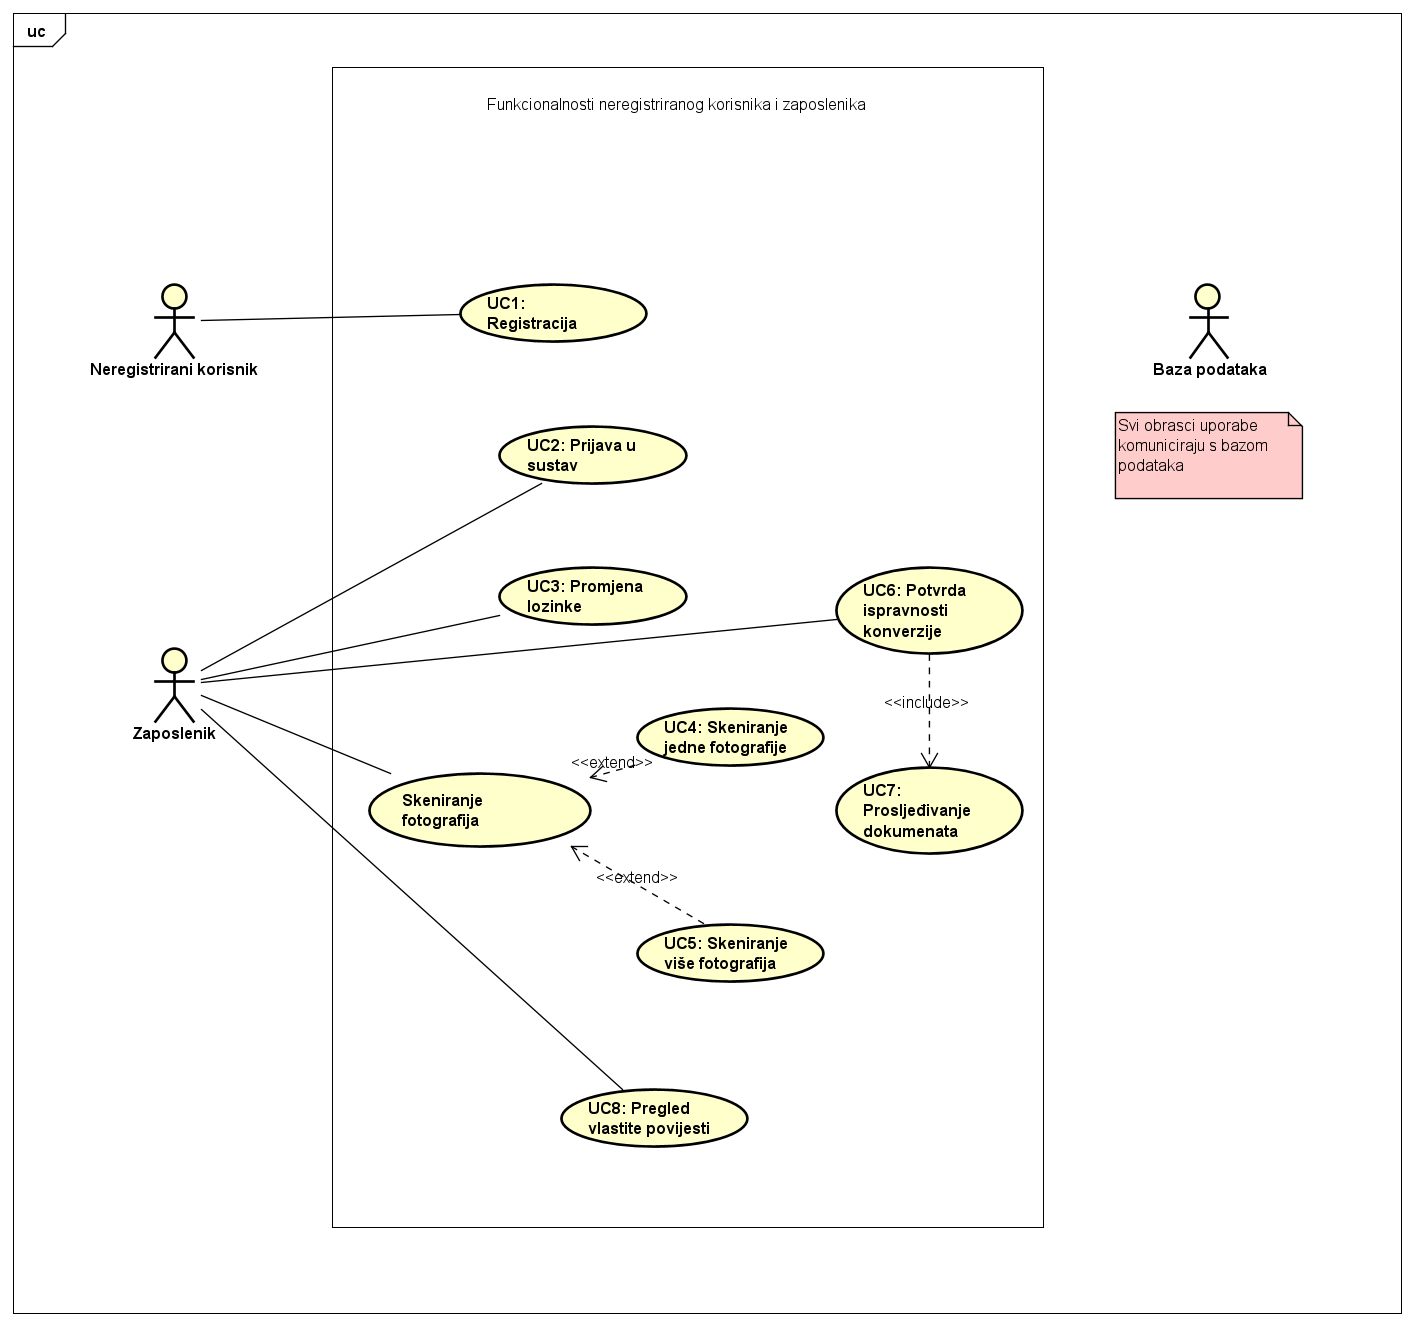
\includegraphics[scale=0.5]{slike/dijagram_obrasca_uporabe_1.PNG} %veličina slike u odnosu na originalnu datoteku i pozicija slike
					\centering
					\caption{Use case dijagram 1}
					\label{fig:promjene}
				\end{figure}
				
				\begin{figure}[H]
					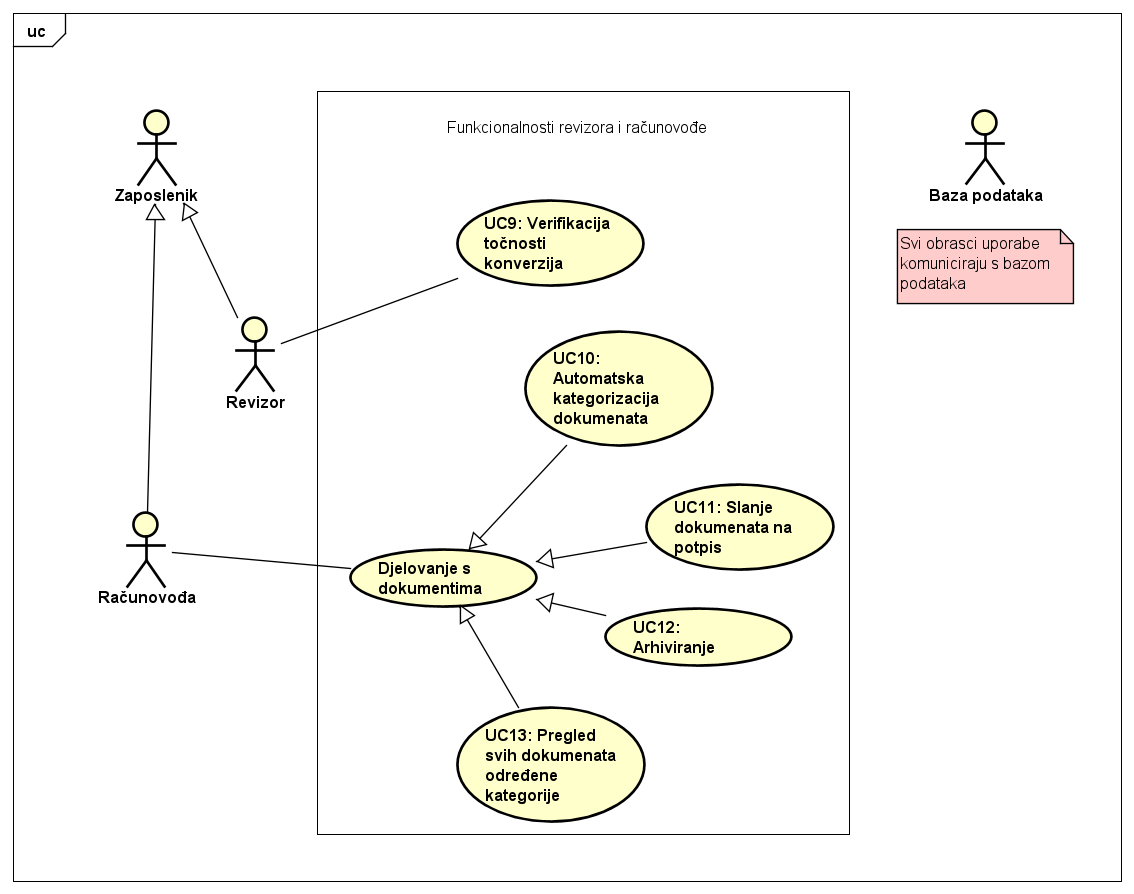
\includegraphics[scale=0.5]{slike/dijagram_obrasca_uporabe_2.PNG} %veličina slike u odnosu na originalnu datoteku i pozicija slike
					\centering
					\caption{Use case dijagram 2}
					\label{fig:promjene}
				\end{figure}		
				
				\begin{figure}[H]
					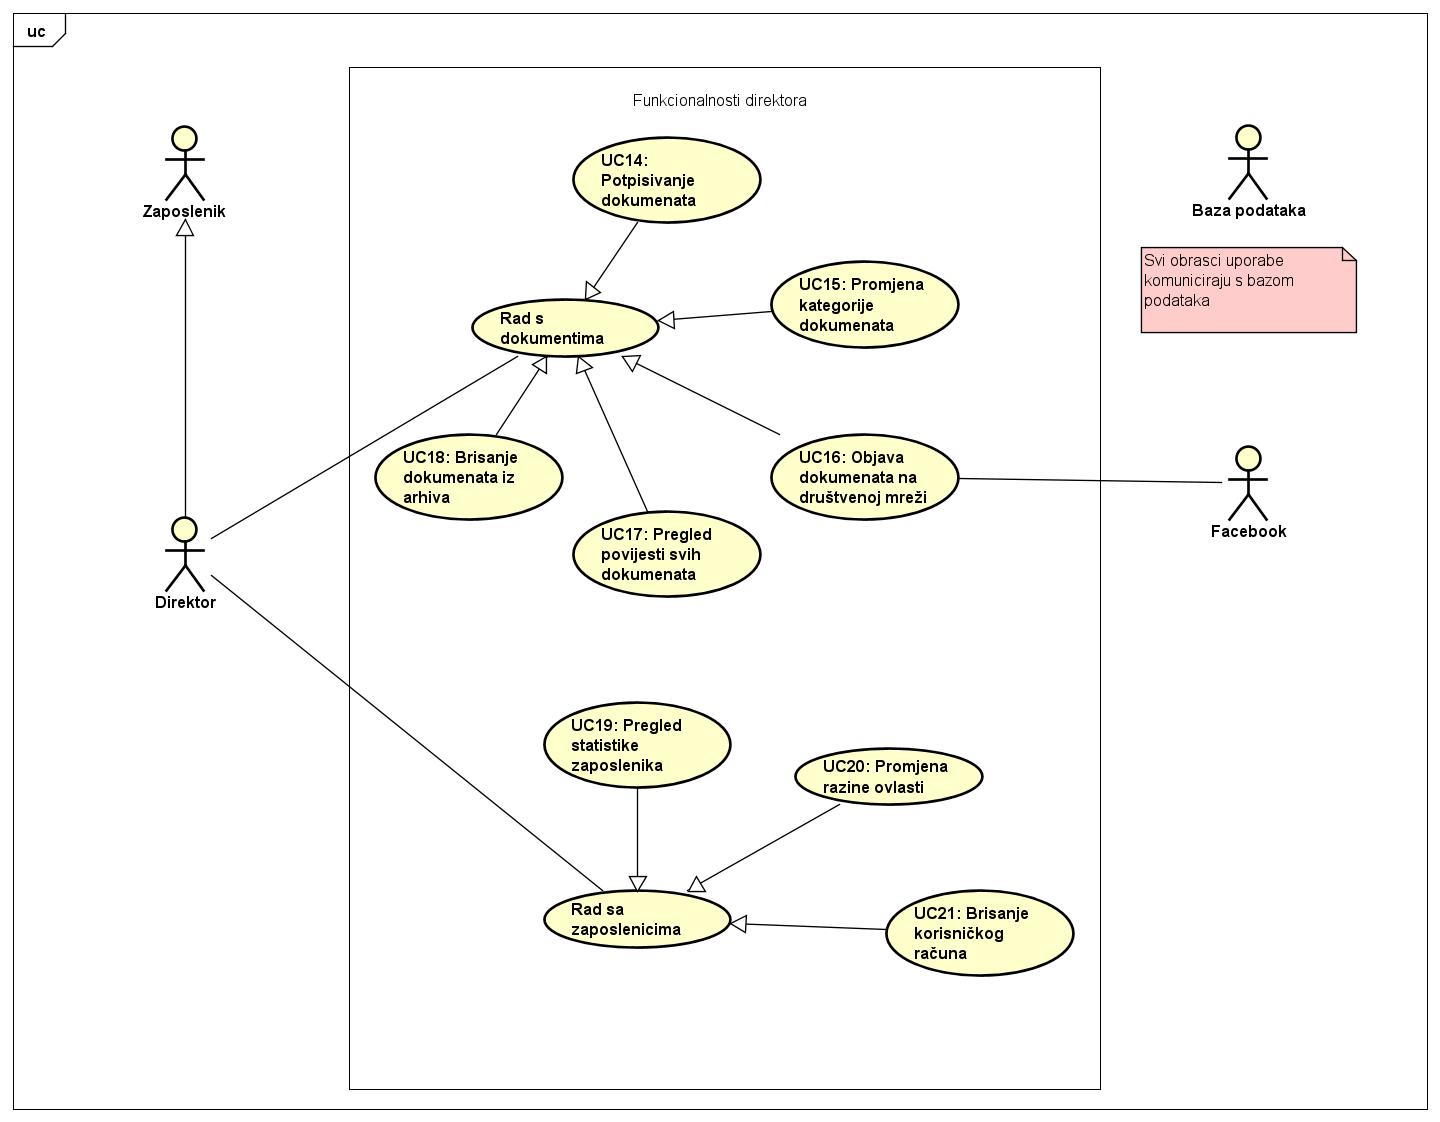
\includegraphics[scale=0.4]{slike/dijagram_obrasca_uporabe_3.PNG} %veličina slike u odnosu na originalnu datoteku i pozicija slike
					\centering
					\caption{Use case dijagram 3}
					\label{fig:promjene}
				\end{figure}
				
			\subsection{Sekvencijski dijagrami}
				
				\begin{figure}[H]
					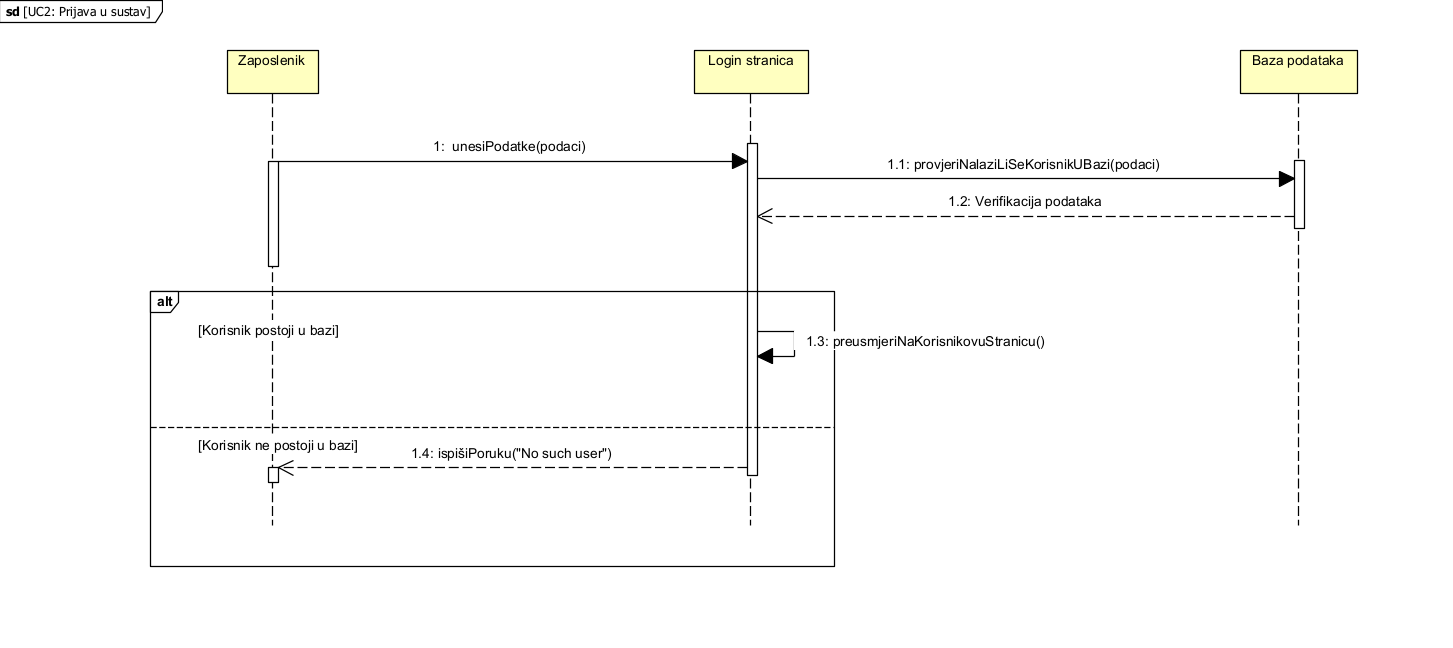
\includegraphics[scale=0.5]{slike/sd1.PNG} %veličina slike u odnosu na originalnu datoteku i pozicija slike
					\centering
					\caption{Sekvencijski dijagram 1 - Login}
					\label{fig:promjene}
				\end{figure}

				\begin{figure}[H]
					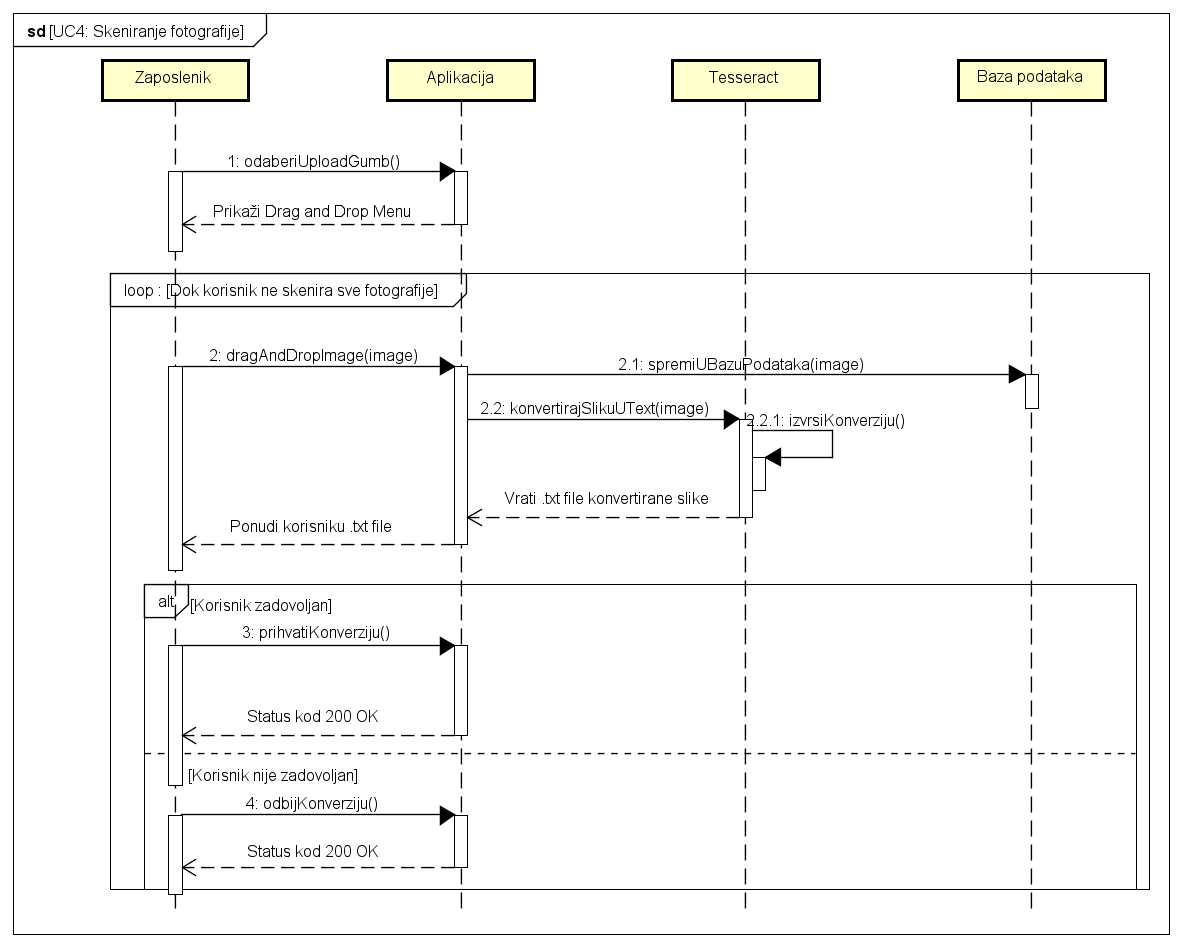
\includegraphics[scale=0.5]{slike/uc4_skeniranje_fotografije.PNG} %veličina slike u odnosu na originalnu datoteku i pozicija slike
					\centering
					\caption{Sekvencijski dijagram 2 - Skeniranje fotografija}
					\label{fig:promjene}
				\end{figure}

				\begin{figure}[H]
					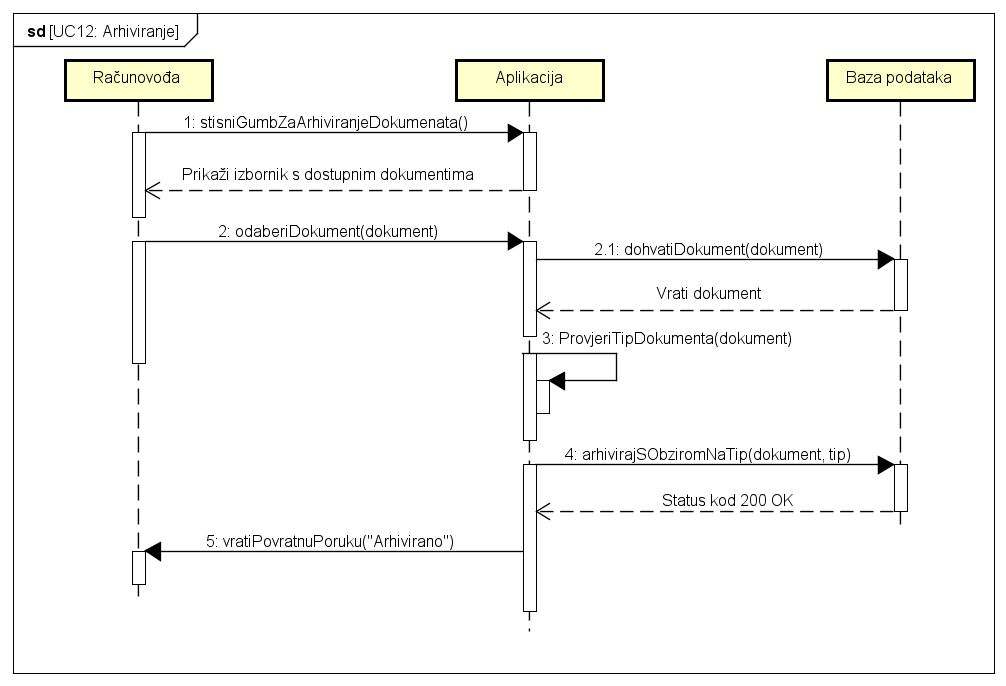
\includegraphics[scale=0.5]{slike/uc12_arhiviranje.PNG} %veličina slike u odnosu na originalnu datoteku i pozicija slike
					\centering
					\caption{Sekvencijski dijagram 3 - Arhiviranje}
					\label{fig:promjene}
				\end{figure}

				\begin{figure}[H]
					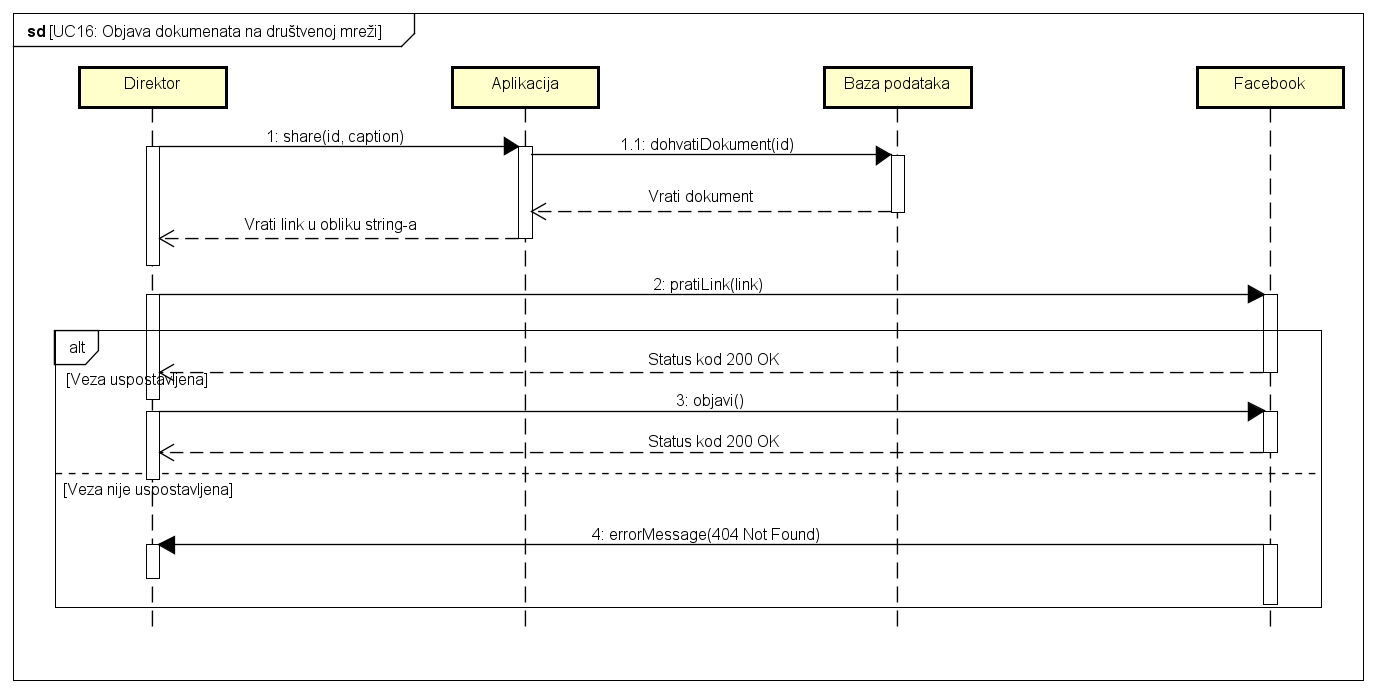
\includegraphics[scale=0.5]{slike/uc16_objava_dokumenata_na_drustvenoj_mrezi.PNG} %veličina slike u odnosu na originalnu datoteku i pozicija slike
					\centering
					\caption{Sekvencijski dijagram 4 - Objava dokumenata na društvenoj mreži}
					\label{fig:promjene}
				\end{figure}
	
		\section{Ostali zahtjevi}
		
		\begin{packed_item}
			\item Korisničko sučelje mora podržavati čitavu hrvatsku abecedu
			
			\item Odgovor na HTTP zahtjev ne smije trajati duže od nekoliko sekundi
			
			\item Aplikacija mora podržati rad više korisnika istovremeno
			
			\item Korisničko sučelje mora biti jasno i jednostavno za upotrebu
			
			\item Sustav mora biti implementiran kao web-aplikacija
			
			\item Sustavu se mora putem HTTPS protokola moći pristupiti s javne mreže
			
			\item Nadogradnja sustava ne smije narušiti postojeće funkcionalnosti
			
			\item Mora postojati mogućnost brze i učinkovite nadogradnje sustava
			
		\end{packed_item}
		
			
			 
			 
			 
	
		\chapter{Arhitektura i dizajn sustava}
		


	
	Arhitektura aplikacije može se podijeliti na 3 djela. 
	
	\begin{packed_item}
		\item web poslužitelj
		
		\item web preglednik
		
		\item baza podataka
	
	\end{packed_item}
	
	\underbar{Web preglednik} je program koji korisniku omogućuje pristup web stranicama te multimedijskom sadržaju na njima. Web preglednik omogućuje korisniku pristup web poslužitelju putem HTTPS (eng. \textit{Hypertext Transfer Protokol Secure}) protokola te interpretira sadržaj kojeg je poslao Web poslužitelj u ljudski razumljiv oblik.
	
	\underbar{Web poslužitelj} je program koji prima i odgovara na korisnikove HTTPS zahtjeve. Web poslužitelj pokreće aplikaciju te korisniku šalje potrebne podatke kako bi korisnikov web preglednik mogao generirati frotnend aplikacije. Frontend predstavlja korisničko sučelje te je pisan u HTML-u, CSS-u i JavaScriptu uz pomoć React framework-a. ReactJS je biblioteka čiji su glavni element komponente. Komponente unutar sebe sadržavaju dijelove korisničkog sučelja te opisuju njihovo ponašanje. Glavna prednost korištenja komponenti je što se one mogu ponovno koristiti te se nove složenije komponente mogu spajati u složenije. Ovakav modularan pristup dizajniranju korisničkog sučelja čini nadogradnju i promjenu korisničkog sučelja vrlo jednostavnom. React dodatno sadrži virtualan DOM kojim optimizira rad korisničkog sučelja tako što minimizira broj manipulacija stvarnog DOM-a. Web poslužitelj je pisan u programskom jeziku Java i Spring Boot radnom okviru. Web poslužitelj komunicira sa bazom podataka te šalje podatke iz nje korisniku u prikladnom obliku. Spring Boot je radno sučelje za brz i učinkovit razvoj WEB aplikacija. Drži se principa konvencija iznad konfiguracije (engl. convention over configuration), to znači da Spring Boot oduzima mogućnost potpuno kontrole nad funkcioniranjem sustava od korisnika no zauzvrat pojednostavljuje razvoj web poslužitelja. Spring Boot ima višeslojnu  arhitekturu gdje se podatci i zahtjevi šalju među raznim slojevima od kojih svaki ima svoju zadaću i logiku. Tako controller sloj prima i obrađuje HTTP zahtijeve, data access sloj komunicira s bazom podataka, exception handling layer je odgovoran za hvatanje i obrađivanje pogreški...
	
	\underbar{Baza podataka} implementirana je putem PostgresSQL-a. Sadrži podatke potrebne za funkcioniranje aplikacije te njihove međusobne odnose. 

	
		

	
				
		\section{Baza podataka}
			
		Baza podataka za web aplikaciju koristi relacijski model podataka. Kao RDBMS (Relational Database Management System) koristi se PostgreSQL verzija 15.0. Koristeći ERDPlus, stvaramo ER dijagram baze podataka u kojem navodimo sve entitete, njihove atribute te međusobne veze. Daljnje tipove podataka, primarne, strane i alternativne ključeve navodimo u relacijskoj shemi baze podataka.
		
			
			\subsection{Opis tablica}
				%\textbf{Employee}]
				Employee  Ovaj entitet sadržava sve važne informacije o zaposleniku koji koristi aplikaciju. Sadrži atribute: id, first\_name, last\_name, email, password i role. Ovaj entitet u vezi je One-to-Many s entitetom Photos preko zaposlenikovog id-a te je u vezi One-to-Many s entitetom Document preko zaposlenikovog id-a.
			
		
				\begin{longtblr}[
					label=none,
					entry=none
					]{
						width = \textwidth,
						colspec={|X[6,l]|X[7, l]|X[20, l]|}, 
						rowhead = 1,
					} %definicija širine tablice, širine stupaca, poravnanje i broja redaka naslova tablice
					\hline \SetCell[c=3]{c}{\textbf{Employee}}	 \\ \hline[3pt]
					\SetCell{LightGreen}id & BIGINT	&  	Jedinstveni identifikator svakog zaposlenika  	\\ \hline
					first\_name	& VARCHAR(255) &   Ime zaposlenika	\\ \hline
                    last\_name & VARCHAR(255) &   Prezime korisnika    \\ \hline 
					role & VARCHAR(255) &   Funkcija svakog zaposlenika (limitirano na Zaposlenik, Revizor, Računovođa i Direktor)   \\ \hline 
					password & VARCHAR(255)	&  	Zaposlenikova hashirana lozinka  	\\ \hline 
					email & VARCHAR(255)   &   E-mail korisnika \\ \hline
				\end{longtblr}
				
				\textbf{Photos}  Ovaj entitet sadržava sve važne informacije o fotografijama pohranjenima u bazu. Sadrži atribute: photoid, url, image\_name, upload\_time te strani ključ upload\_employee\_id preko korisnika. Ovaj entitet u vezi je Many-to-One s entitetom Employee preko zaposlenikovog id-a te je u One-to-One vezi s entitetom Document koji sadrži strani ključ photo\_id.

				\begin{longtblr}[
					label=none,
					entry=none
					]{
						width = \textwidth,
						colspec={|X[11,l]|X[8, l]|X[20, l]|}, 
						rowhead = 1,
					}
					\hline \SetCell[c=3]{c}{\textbf{Photos}}	 \\ \hline[3pt]
					\SetCell{LightBlue} upload\_employee\_id	& BIGINT   &   Jedinstveni identifikator zaposlenika koji je objavio fotografiju izveden iz tablice Employee	\\ \hline
                    \SetCell{LightGreen} photo\_id  & BIGINT   &   Jedinstveni identifikator fotografije \\ \hline
                    url   & VARCHAR(255)   &  URL fotografije \\ \hline
                    image\_name   & VARCHAR(255)  &  Ime prenesene fotografije \\ \hline
                    upload\_time  & TIMESTAMP  &  Datum i vrijeme prijenosa fotografije \\ \hline
				\end{longtblr}

				\textbf{Document}  Ovaj entitet sadržava sve važne informacije o dokumentima pohranjenima u bazi. Sadrži atribute: id, correct, type, to\_be\_signed, signed, verified, url, file\_name te strane ključeve photo\_id, scan\_employee\_id i verification\_employee\_id. Ovaj entitet u vezi je One-to-One s entitetom Photos preko photo\_id, u Many-to-One vezi je s entitetom Employee te je u vezi One-to-One s entitetom Archive koji sadrži document\_id kao strani ključ.

                \begin{longtblr}[
					label=none,
					entry=none
					]{
						width = \textwidth,
						colspec={|X[17,l]|X[10, l]|X[20, l]|}, 
						rowhead = 1,
					}
					\hline \SetCell[c=3]{c}{\textbf{Document}}	 \\ \hline[3pt]
                    \SetCell{LightBlue} photo\_id  &  BIGINT  &  Jedinstveni identifikator fotografije sadržane u dokumentu, izveden iz tablice Photos	\\ \hline
					\SetCell{LightBlue} scan\_employee\_id  &  BIGINT  &  Jedinstveni identifikator zaposlenika koji je skenirao dokument izveden iz tablice Employee	\\ \hline
					\SetCell{LightBlue} verification\_employee\_id  &  BIGINT  &  Jedinstveni identifikator zaposlenika zaduženog za verifikaciju ispravnosti konverzije, izveden iz tablice Employee	\\ \hline
                    \SetCell{LightGreen} id  &  BIGINT  &  Jedinstveni identifikator prenesenog dokumenta \\ \hline
                    correct  &  BOOLEAN  &  Potvrda ukoliko je rezultantni dokument ispravno skeniran \\ \hline
                    type  &  VARCHAR(255)  &  Tip dokumenta (limitirano na Račun, Ponuda i Interni dokument) \\ \hline
                    signed  &  BOOLEAN  &  Potvrda ukoliko je rezultantni dokument potpisan od strane direktora \\ \hline
                    verified  &  BOOLEAN  &  Potvrda ukoliko je rezultantni dokument potpisan od strane računovođe \\ \hline
                    to\_be\_signed  &  BOOLEAN  &  Potvrda ukoliko rezultantni dokument očekiva potpis od direktora\\ \hline
					file\_name  &  VARCHAR(255)  &  Ime pohranjenog dokumenta\\ \hline
					url  &  VARCHAR(255)  &  URL zapis\\ \hline
                \end{longtblr}

				\textbf{Archive\_entity}  Ovaj entitet sadržava sve važne informacije o arhiviranim dokumentima u bazi. Sadrži atribute: id te strani ključ document\_id preko entiteta Dokument. Ovaj entitet u vezi je One-to-One s entitetom Dokument preko dokumentovog id-a.

                \begin{longtblr}[
					label=none,
					entry=none
					]{
						width = \textwidth,
						colspec={|X[6,l]|X[6, l]|X[20, l]|}, 
						rowhead = 1,
					}
					\hline \SetCell[c=3]{c}{\textbf{Archive}}	 \\ \hline[3pt]
                    \SetCell{LightBlue} document\_id  &  BIGINT  &  Jedinstveni identifikator dokumenta koji se arhivira \\ \hline
                    \SetCell{LightGreen} id  &  BIGINT  &  Jedinstveni identifikator dokumenta koji se nalazi u arhivi \\ \hline
                \end{longtblr}

				\textbf{Login\_log\_out\_record}  Ovaj entitet sadržava sve važne informacije o vremenu rada svakog pojedinačnog zaposlenika. Sadrži atribute: id, login\_time, logout\_time te strani ključ employee\_id preko korisnikovog identifikatora. Ovaj entitet je u vezi Many-to-One s entitetom Employee preko zaposlenikovog id-a.

				\begin{longtblr}[
					label=none,
					entry=none
					]{
						width = \textwidth,
						colspec={|X[6,l]|X[6, l]|X[20, l]|}, 
						rowhead = 1,
					}
					\hline \SetCell[c=3]{c}{\textbf{Login/Logout records}}	 \\ \hline[3pt]
                    \SetCell{LightBlue} employee\_id  &  BIGINT  &  Jedinstveni identifikator zaposlenika čija se aktivnost na stranici sprema u statistiku \\ \hline
					\SetCell{LightGreen} id  &  BIGINT  &  Jedinstveni identifikator session-a koji se gleda \\ \hline
                    login\_time  &  TIMESTAMP  &  Datum i vrijeme login-a zaposlenika \\ \hline
					logout\_time &  TIMESTAMP  &  Datum i vrijeme logout-a zaposlenika \\ \hline
                \end{longtblr}

			\subsection{Dijagram baze podataka}
				
				\begin{figure}[H]
					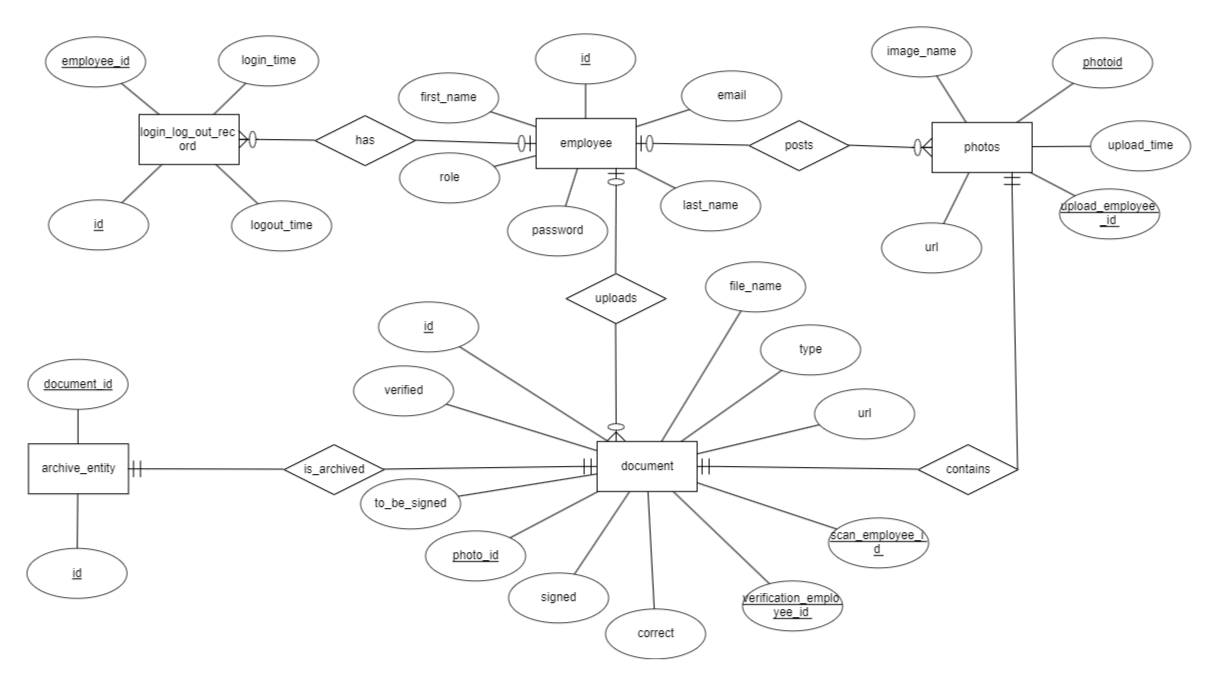
\includegraphics[scale=0.4]{slike/kompletici_v4_ER.png} %veličina slike u odnosu na originalnu datoteku i pozicija slike
					\centering
					\caption{ER dijagram baze podataka}
					\label{fig:promjene}
				\end{figure}
				
					\begin{figure}[H]
					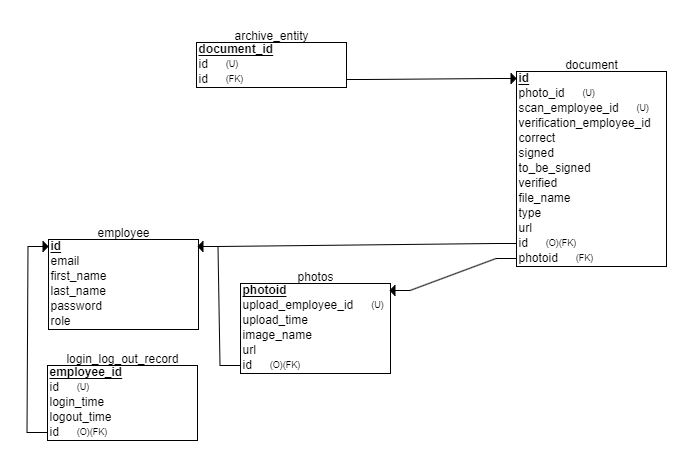
\includegraphics[scale=0.5]{slike/kompletici_v4_REL.PNG} %veličina slike u odnosu na originalnu datoteku i pozicija slike
					\centering
					\caption{REL dijagram baze podataka}
					\label{fig:promjene}
				\end{figure}
				
				
			
			\eject
			
			
		\section{Dijagram razreda}

		Na slikama su prikazani razredi koji pripadaju backend dijelu arhitekture. Na slikama su prikazani razredi koji nasljeđuju Controller razred, metode pomoću kojih oni manipuliraju s DTO (Data transfer objects), te razredi koji implementiraju razred Entity.
		
			\begin{figure}[H]
				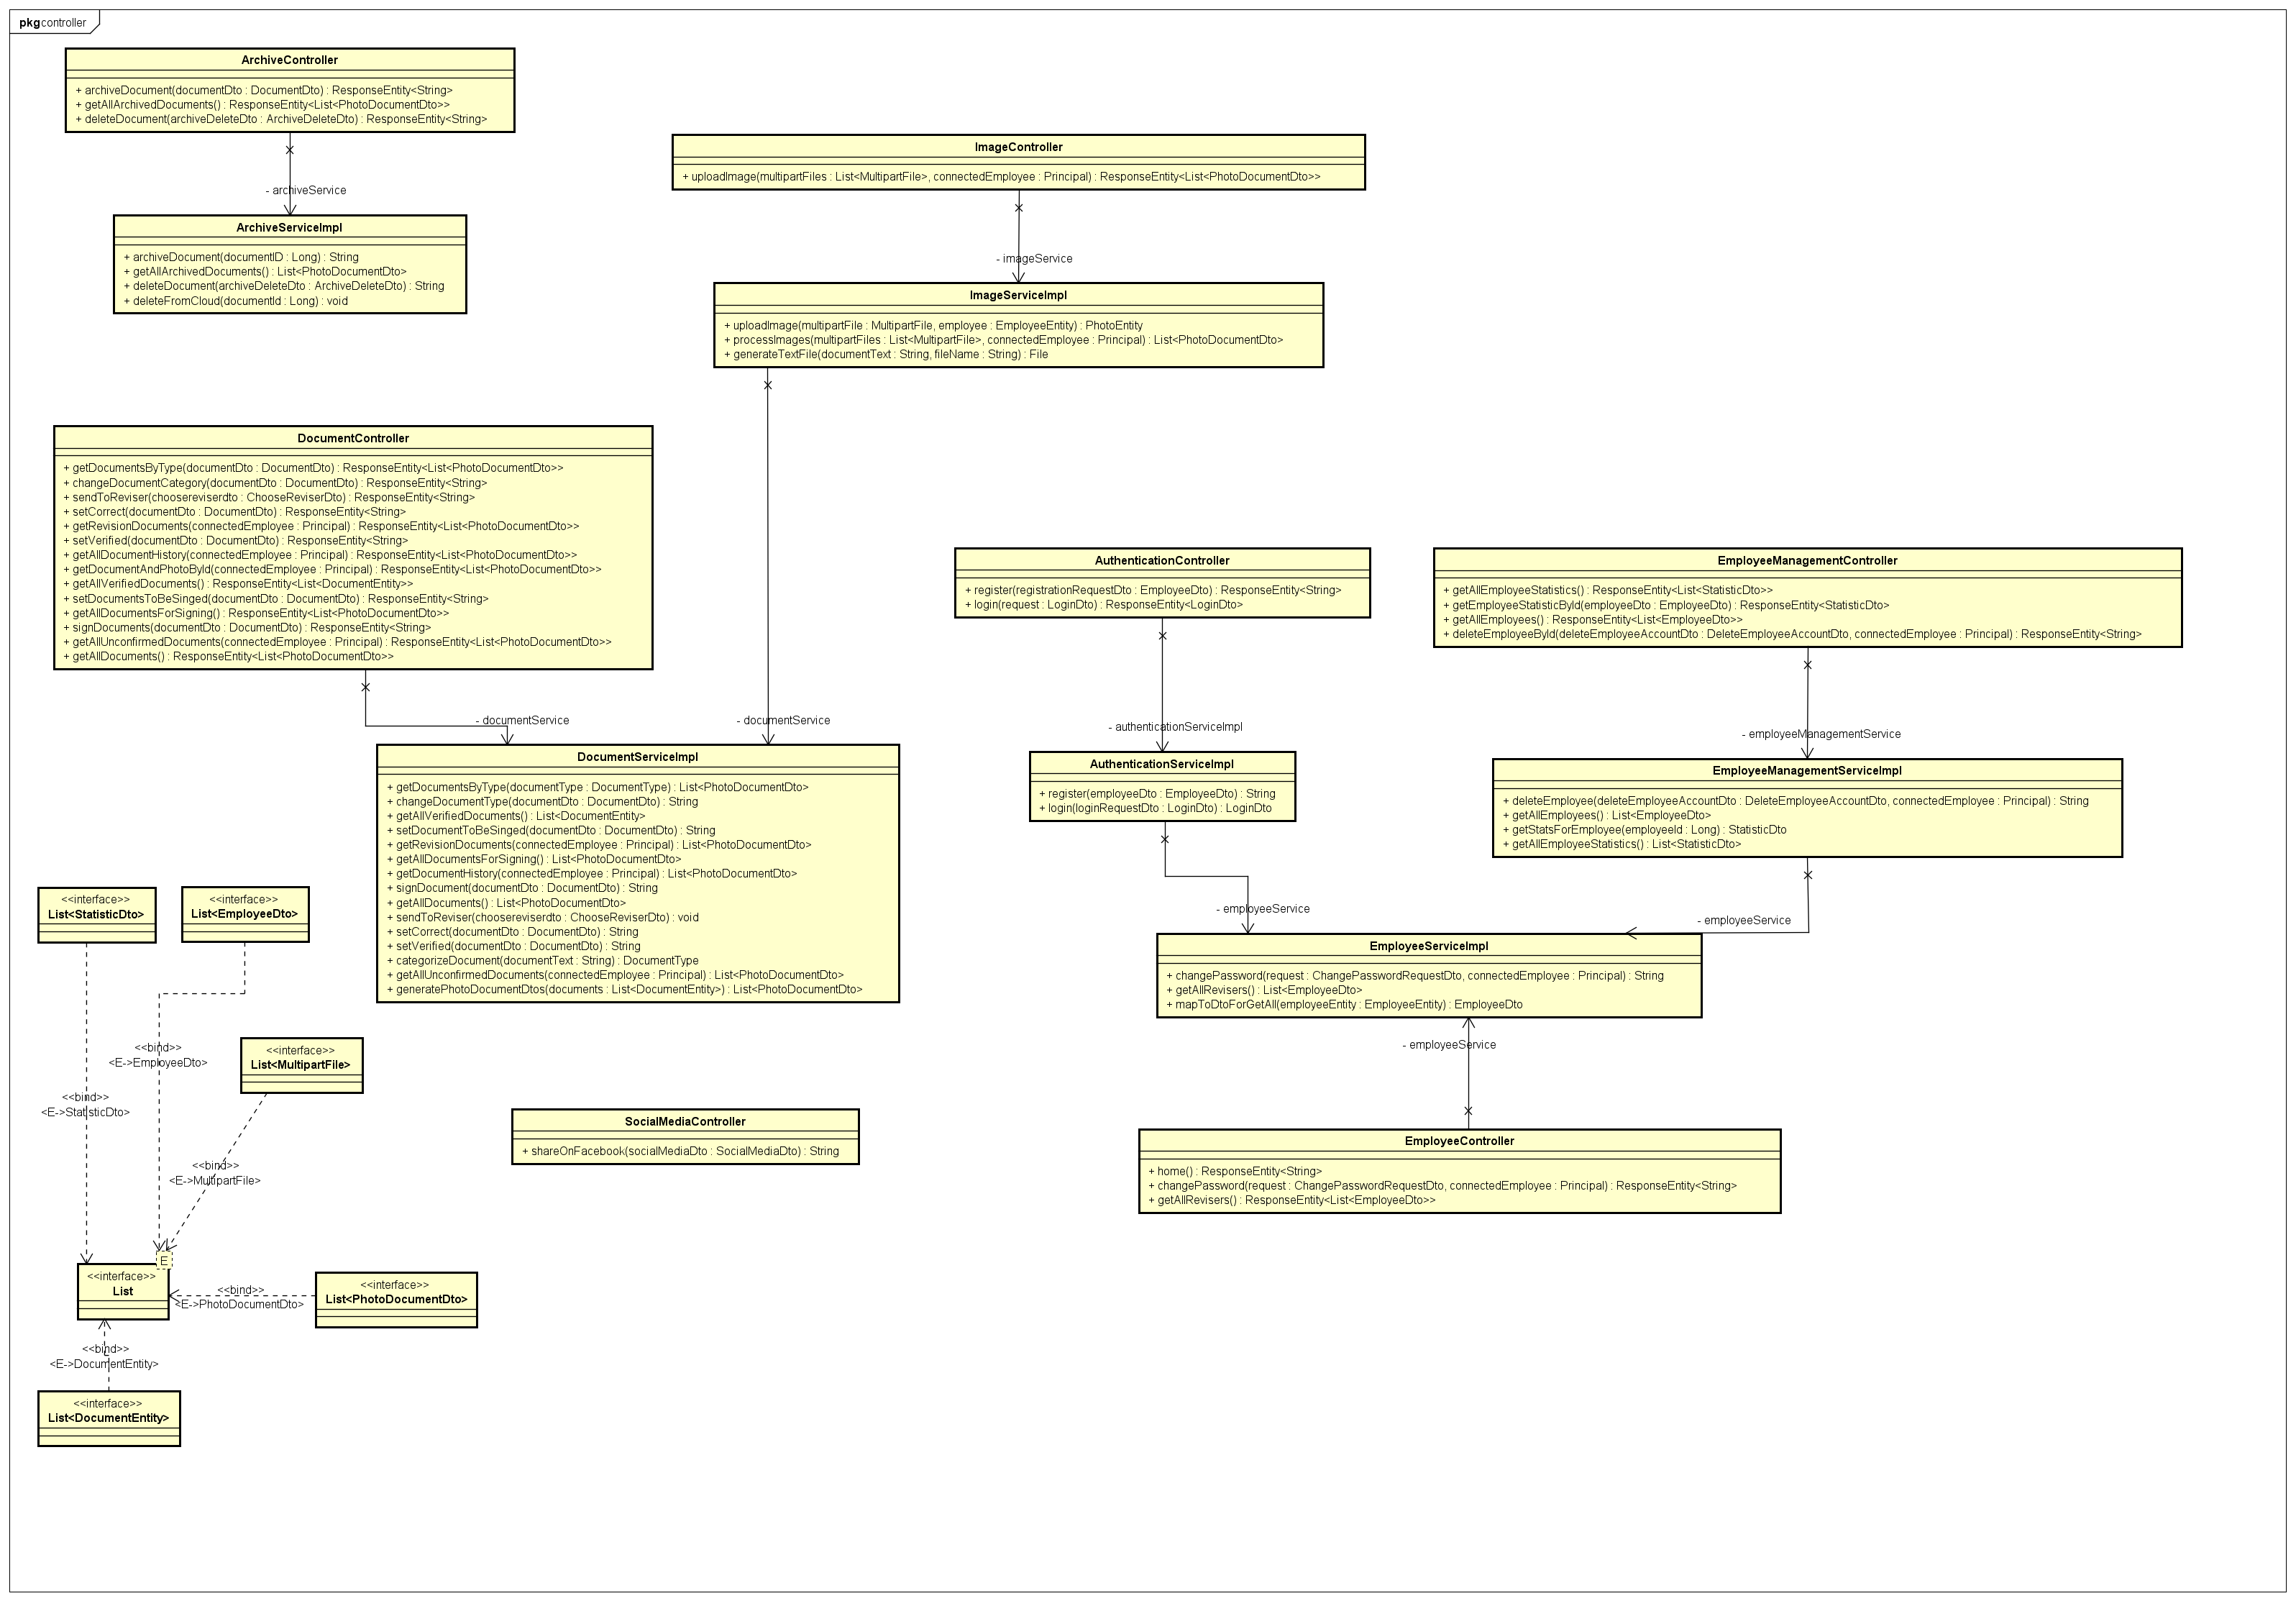
\includegraphics[scale=0.2]{slike/ControlerDiagram.png} %veličina slike u odnosu na originalnu datoteku i pozicija slike
				\centering
				\caption{Dijagram razreda - dio Controllers}
				\label{fig:promjene}
			\end{figure}
			
			\begin{figure}[H]
				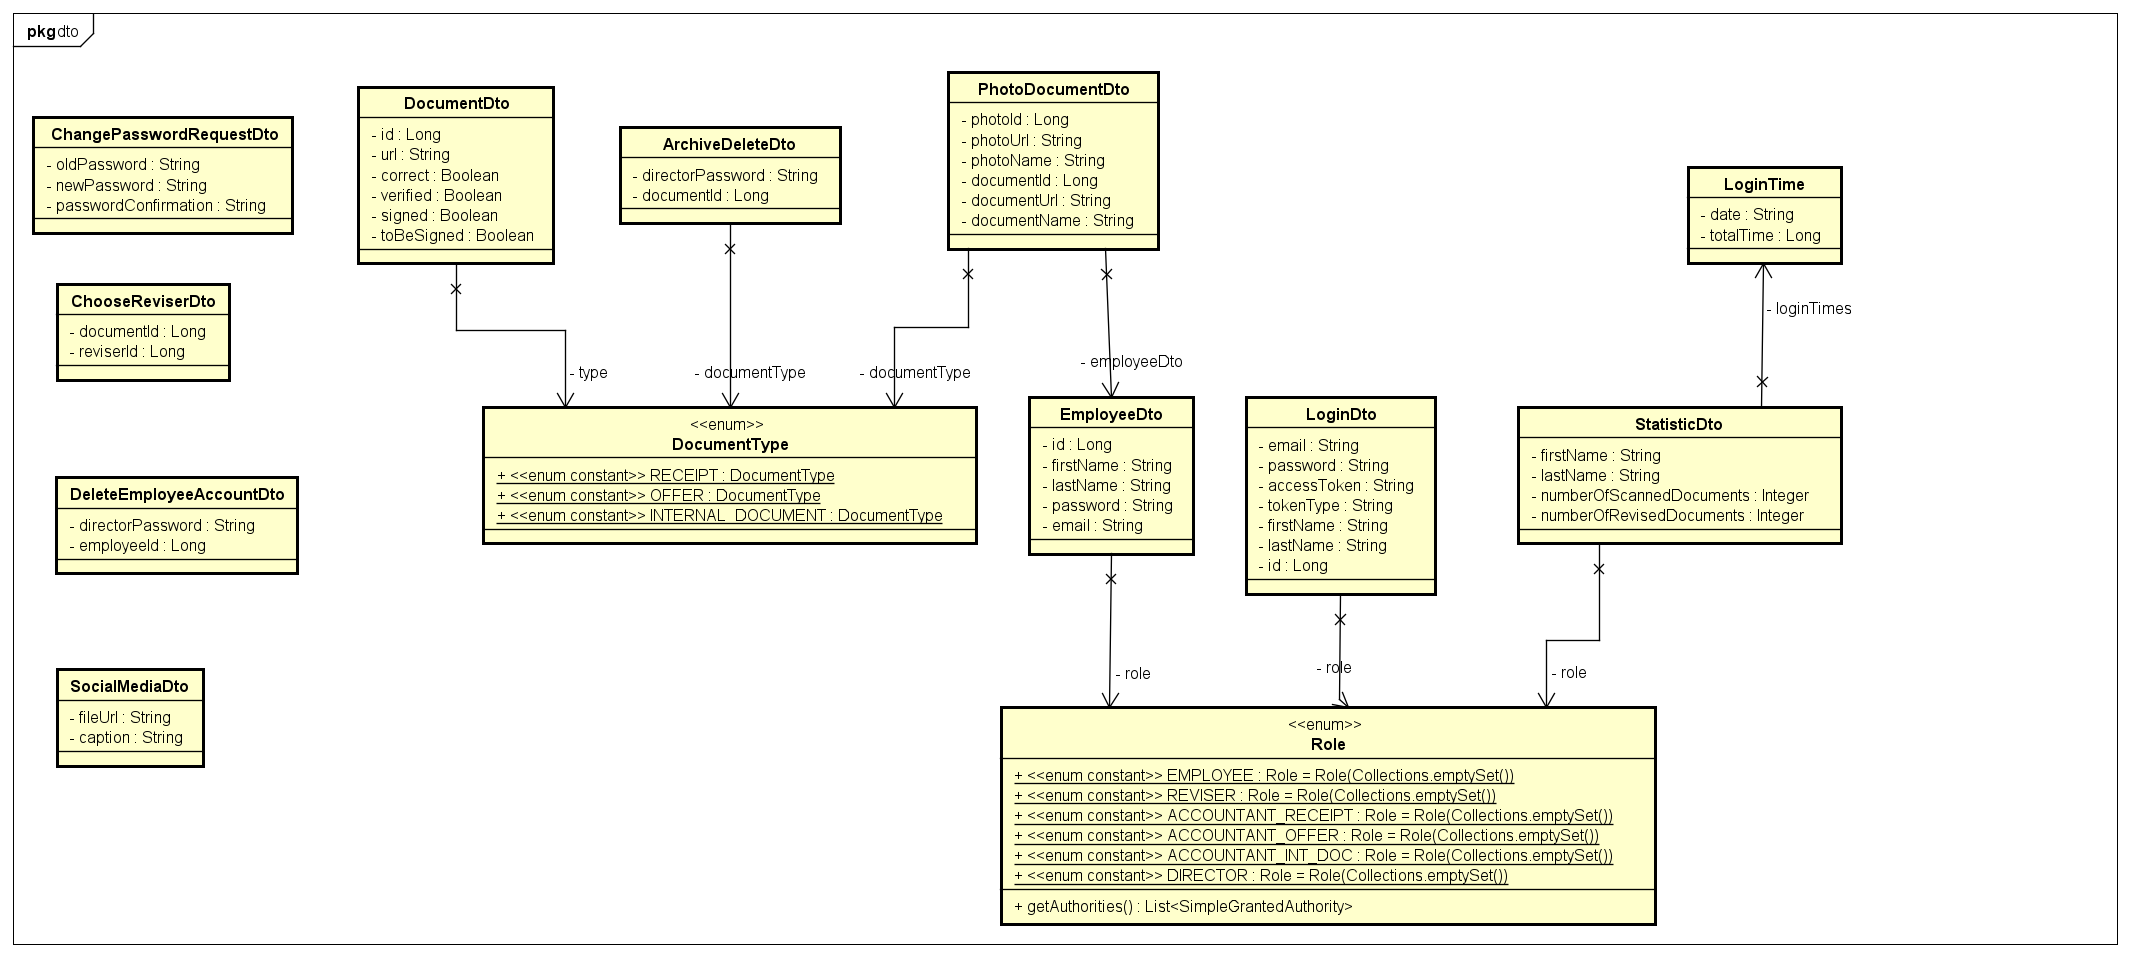
\includegraphics[scale=0.3]{slike/DtoDiagram.png} %veličina slike u odnosu na originalnu datoteku i pozicija slike
				\centering
				\caption{Dijagram razreda - dio Data transfer objects}
				\label{fig:promjene}
			\end{figure}

			\begin{figure}[H]
				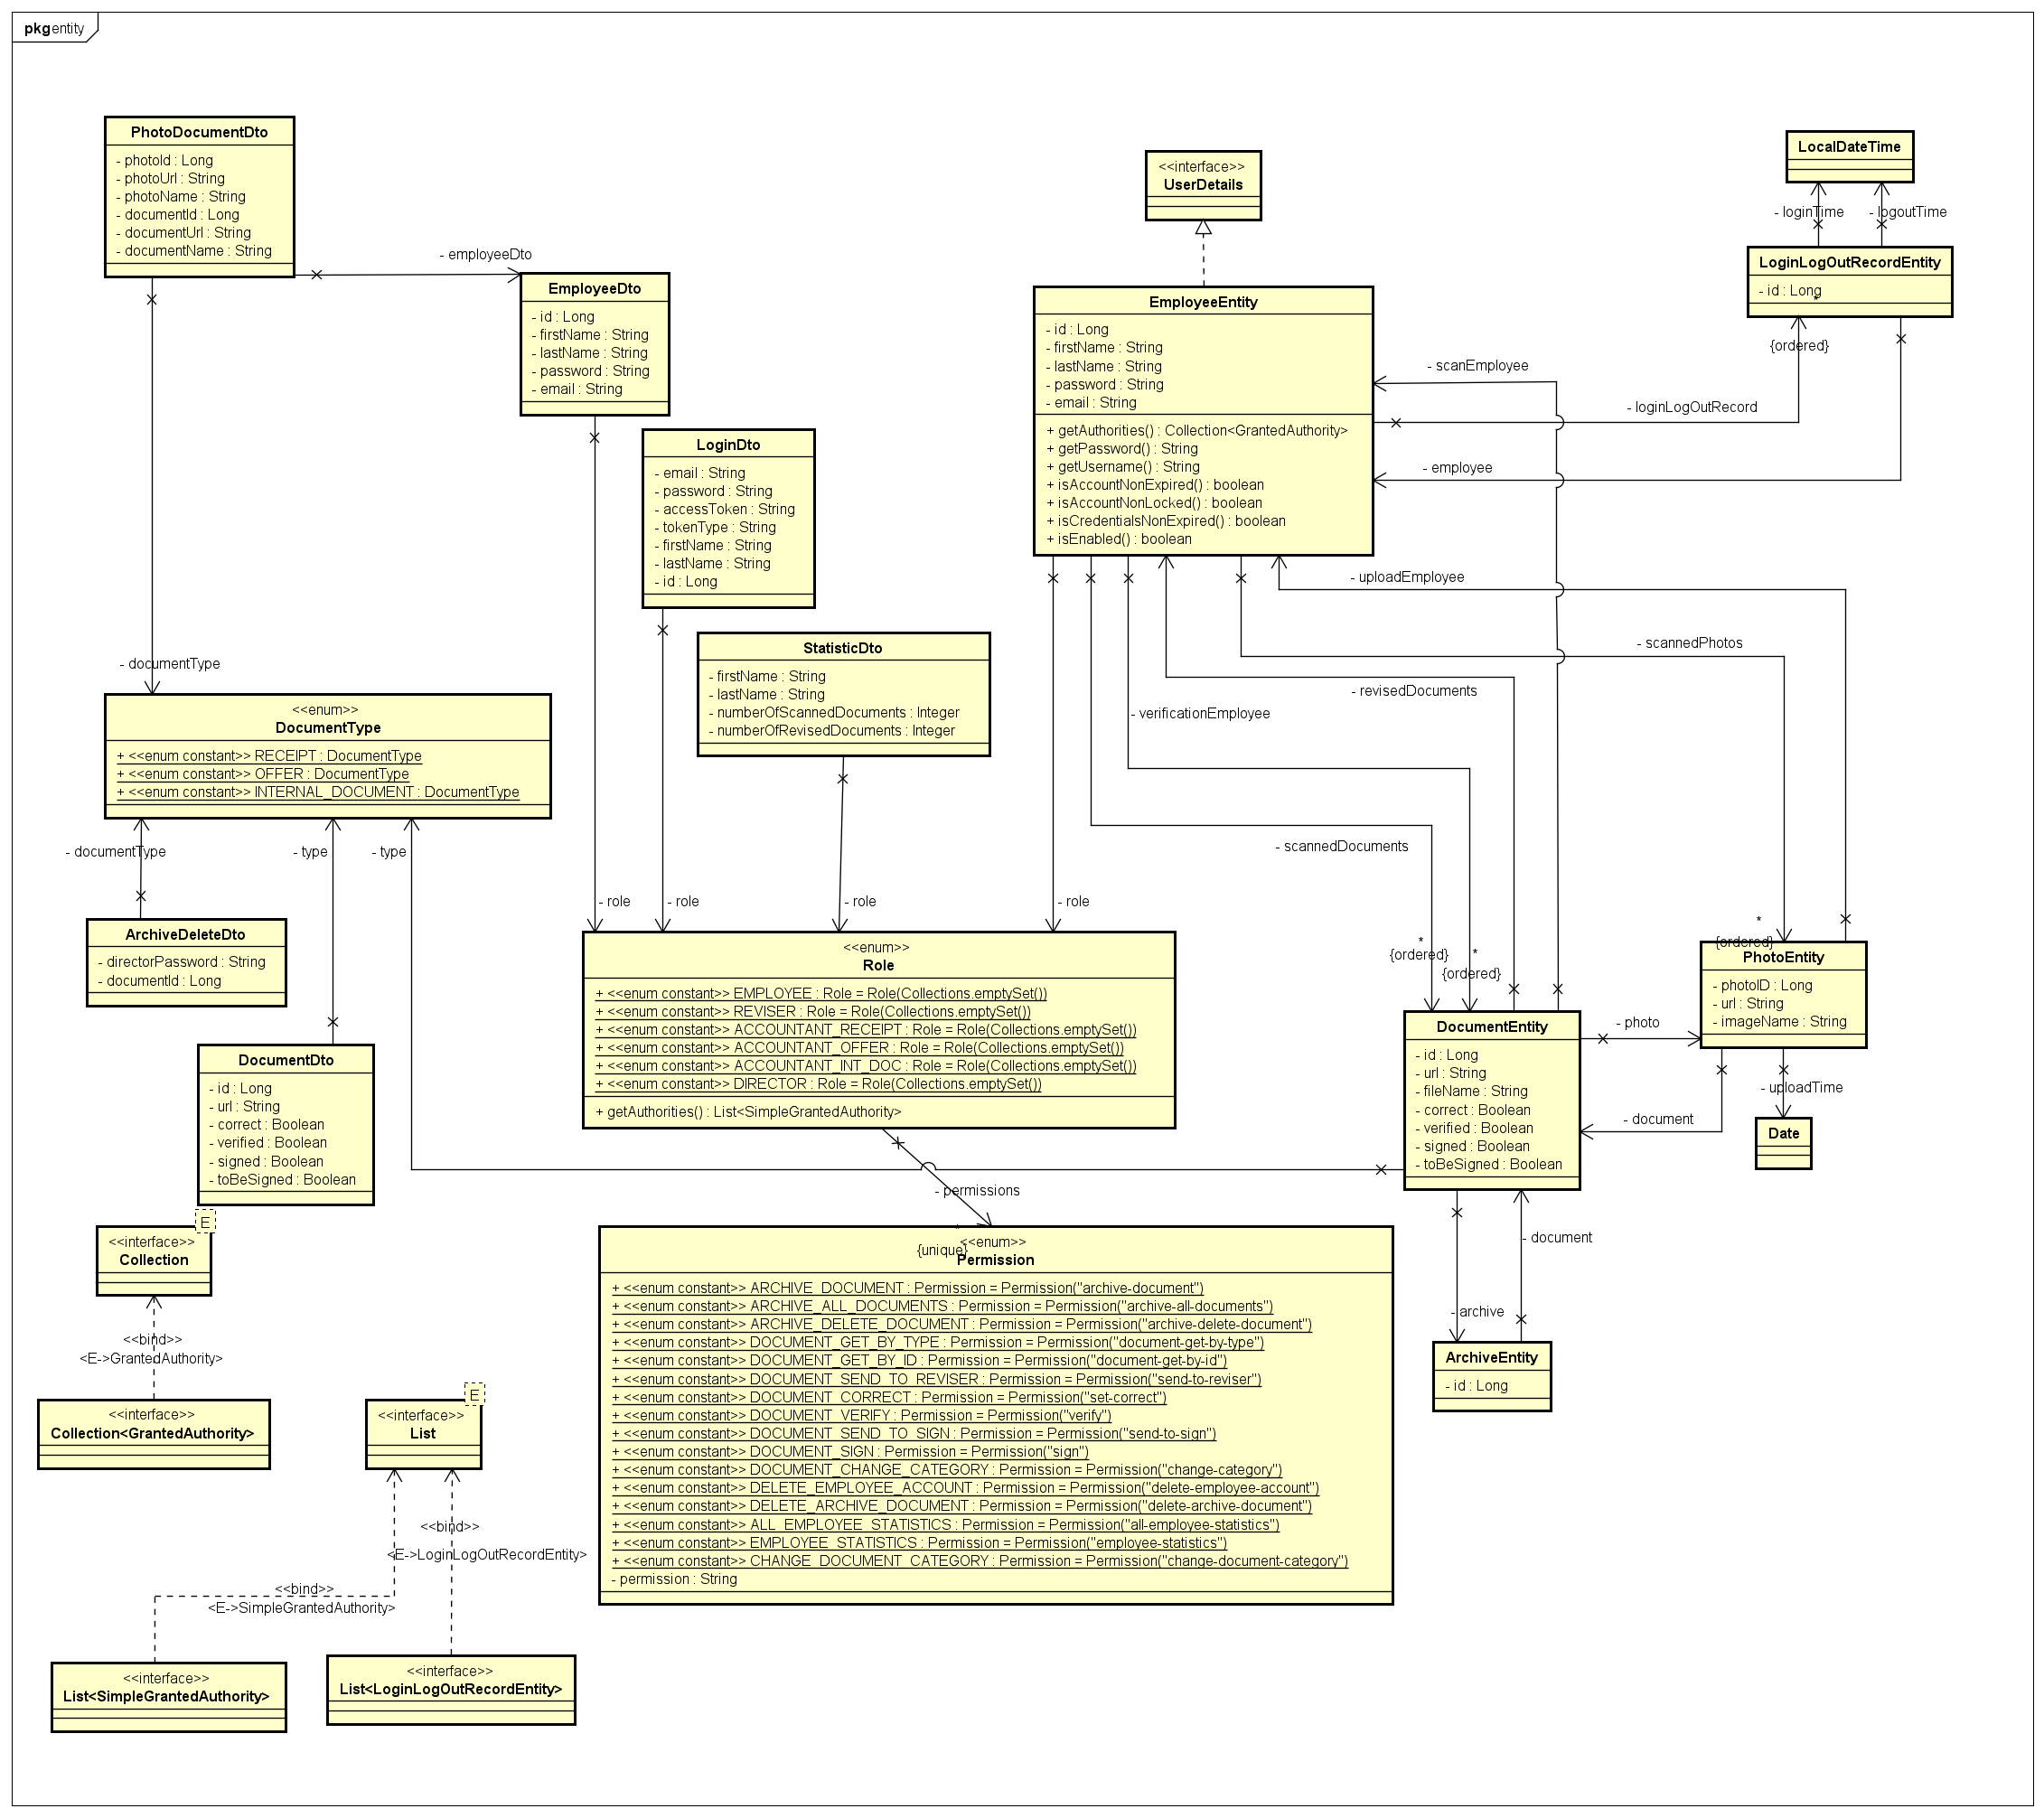
\includegraphics[scale=0.3]{slike/EntityDiagram.png} %veličina slike u odnosu na originalnu datoteku i pozicija slike
				\centering
				\caption{Dijagram razreda - dio Entity}
				\label{fig:promjene}
			\end{figure}
			
			
			
			\eject
		

		\section{Dijagram stanja}
			
			Dijagram stanja prikazuje stanja objekta te prijelaze iz jednog stanja u drugo temeljene na dogadajima. Na slici je prikazan dijagram stanja za direktora. Nakon prijave, direktoru se prikazuje početna stranica na kojoj može pristupit svim svojim funkcionalnostima (skeniranju dokumenata, promjeni lozinke, pregledu zahtjeva itd.). Odabirom na skeniranje dokumenata direktoru se pruža mogućnost odabira upload-a dokumenta ili provjere već dostupnog dokumenta. Odabirom pregleda zahtjeva pružaju mu se opcije revizije, potpisivanja te arhiviranja dokumenta. Odabirom pregleda zapisa direktor može pregledati arhivu, povijest skeniranja te statistiku svih pojedinačnih zaposlenika. Direktoru se također pružaju opcije promjene lozinke, brisanja zaposlenika te objave dokumenta na društvenim mrežama (u ovom slučaju na društvenoj mreži "Facebook").
			
			\begin{figure}[H]
				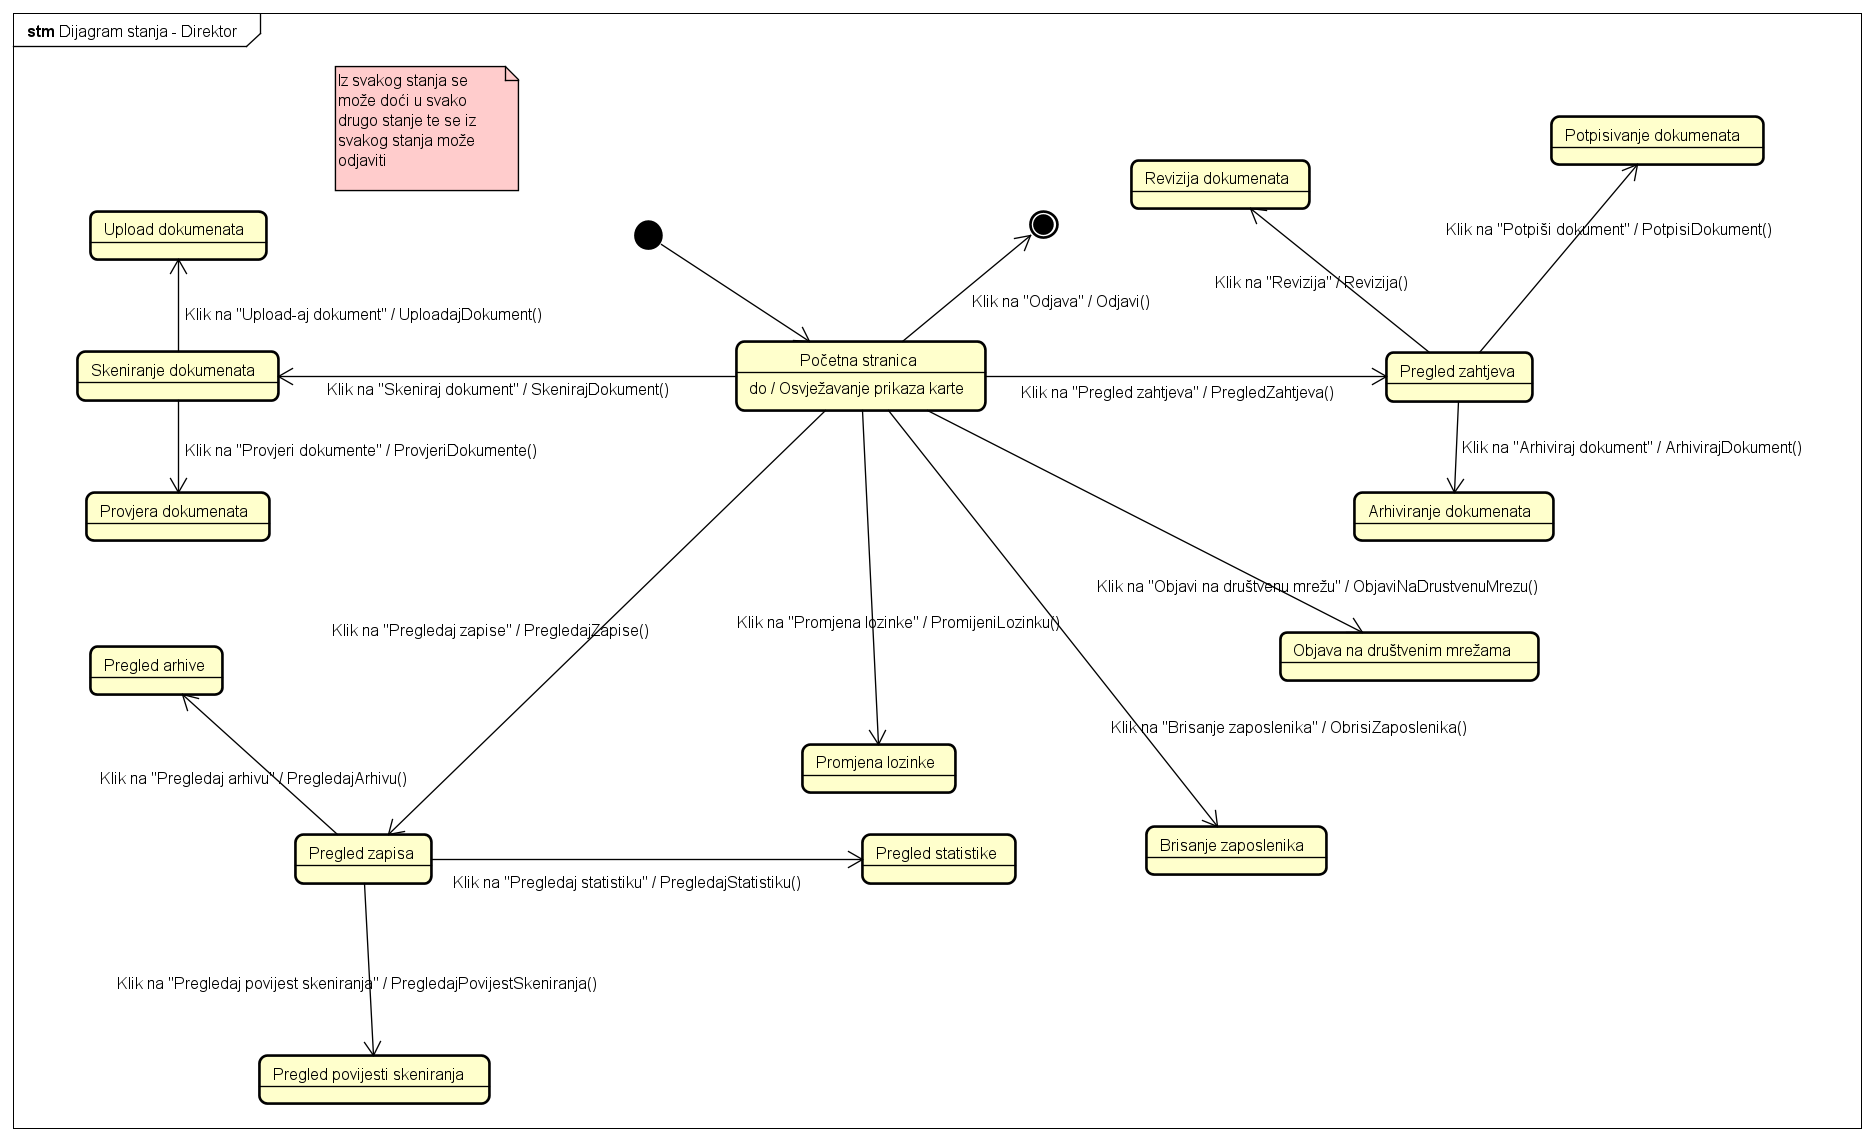
\includegraphics[scale=0.35]{slike/DijagramStanja - Direktor.png} %veličina slike u odnosu na originalnu datoteku i pozicija slike
				\centering
				\caption{Dijagram stanja}
				\label{fig:promjene}
			\end{figure}

			\eject 
		
		\section{Dijagram aktivnosti}
			
			
			Dijagram aktivnosti primjenjuje se za opis modela toka upravljanja ili toka podataka. Ne upotrebljava se za modeliranje događajima poticanog ponašanja. U modeliranju toka upravljanja svaki novi korak poduzima se nakon završenog prethodnog, a naglasak je na jednostavnosti. Na dijagramu aktivnosti prikazan je princip rada zaposlenika. Zaposlenik nakon uspješne prijave u sustav upload-a fotografije koje se daju na skeniranje, te aplikacija iste fotografije konvertira koristeći Tesseract.

			\begin{figure}[H]
				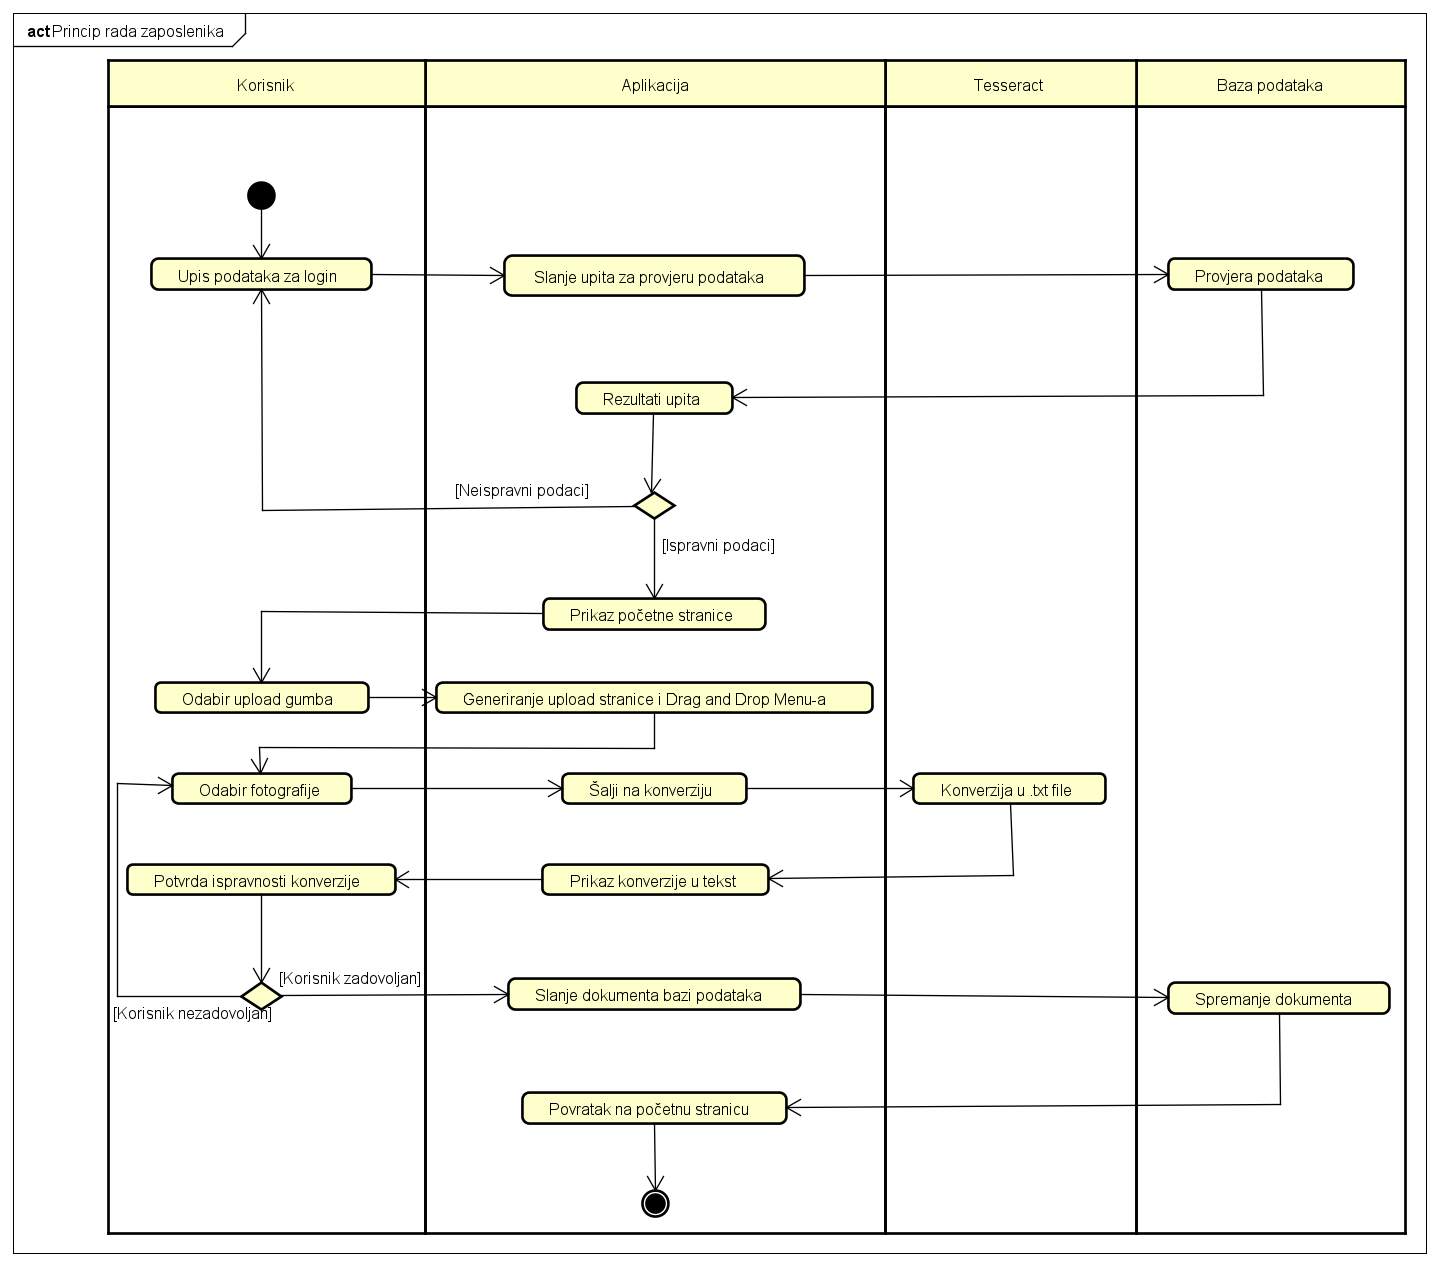
\includegraphics[scale=0.4]{slike/dijagram_aktivnosti.png} %veličina slike u odnosu na originalnu datoteku i pozicija slike
				\centering
				\caption{Dijagram aktivnosti}
				\label{fig:promjene}
			\end{figure}


			\eject
		\section{Dijagram komponenti}
		
			
			 Dijagram komponenti prikazan na slici opisuje organizaciju i međuovisnost komponenti, interne strukture i odnose prema okolini. Sustavu se pristupa preko dva različita sučelja. Preko sučelja za dohvat HTML, CSS i JS datoteka poslužuju se datoteke koje pripadaju frontend dijelu aplikacije. Router je komponenta koja na upit s url određuje koja datoteka će se poslužiti na sučelje. Frontend dio se sastoji od niza JavaScript datoteka koje su raspoređene u logičke cjeline nazvane po tipovima aktora koji im pristupaju. Sve JavaScript datoteke ovise o React biblioteci iz koje dohvaćaju gotove komponente kao što su gumbi, forme i slično. Preko sučelja za dohvat JSON podataka pristupa se REST API komponenti. REST API poslužuje podatke koji pripadaju backend dijelu aplikacije. EntityFrameWorkCore je zadužen za dohvaćanje tablica iz baze podataka pomoću SQL upita. Podaci koji su pristigli iz baze se šalju dalje MVC arhitekturi u obliku DTO preko Services. React-view komponenta preko dostupnih sučelja komunicira sa aplikacijom te ovisno o korisnikovim akcijama osvježava prikaz i dohvaća nove podatke ili datoteke.

			 \begin{figure}[H]
				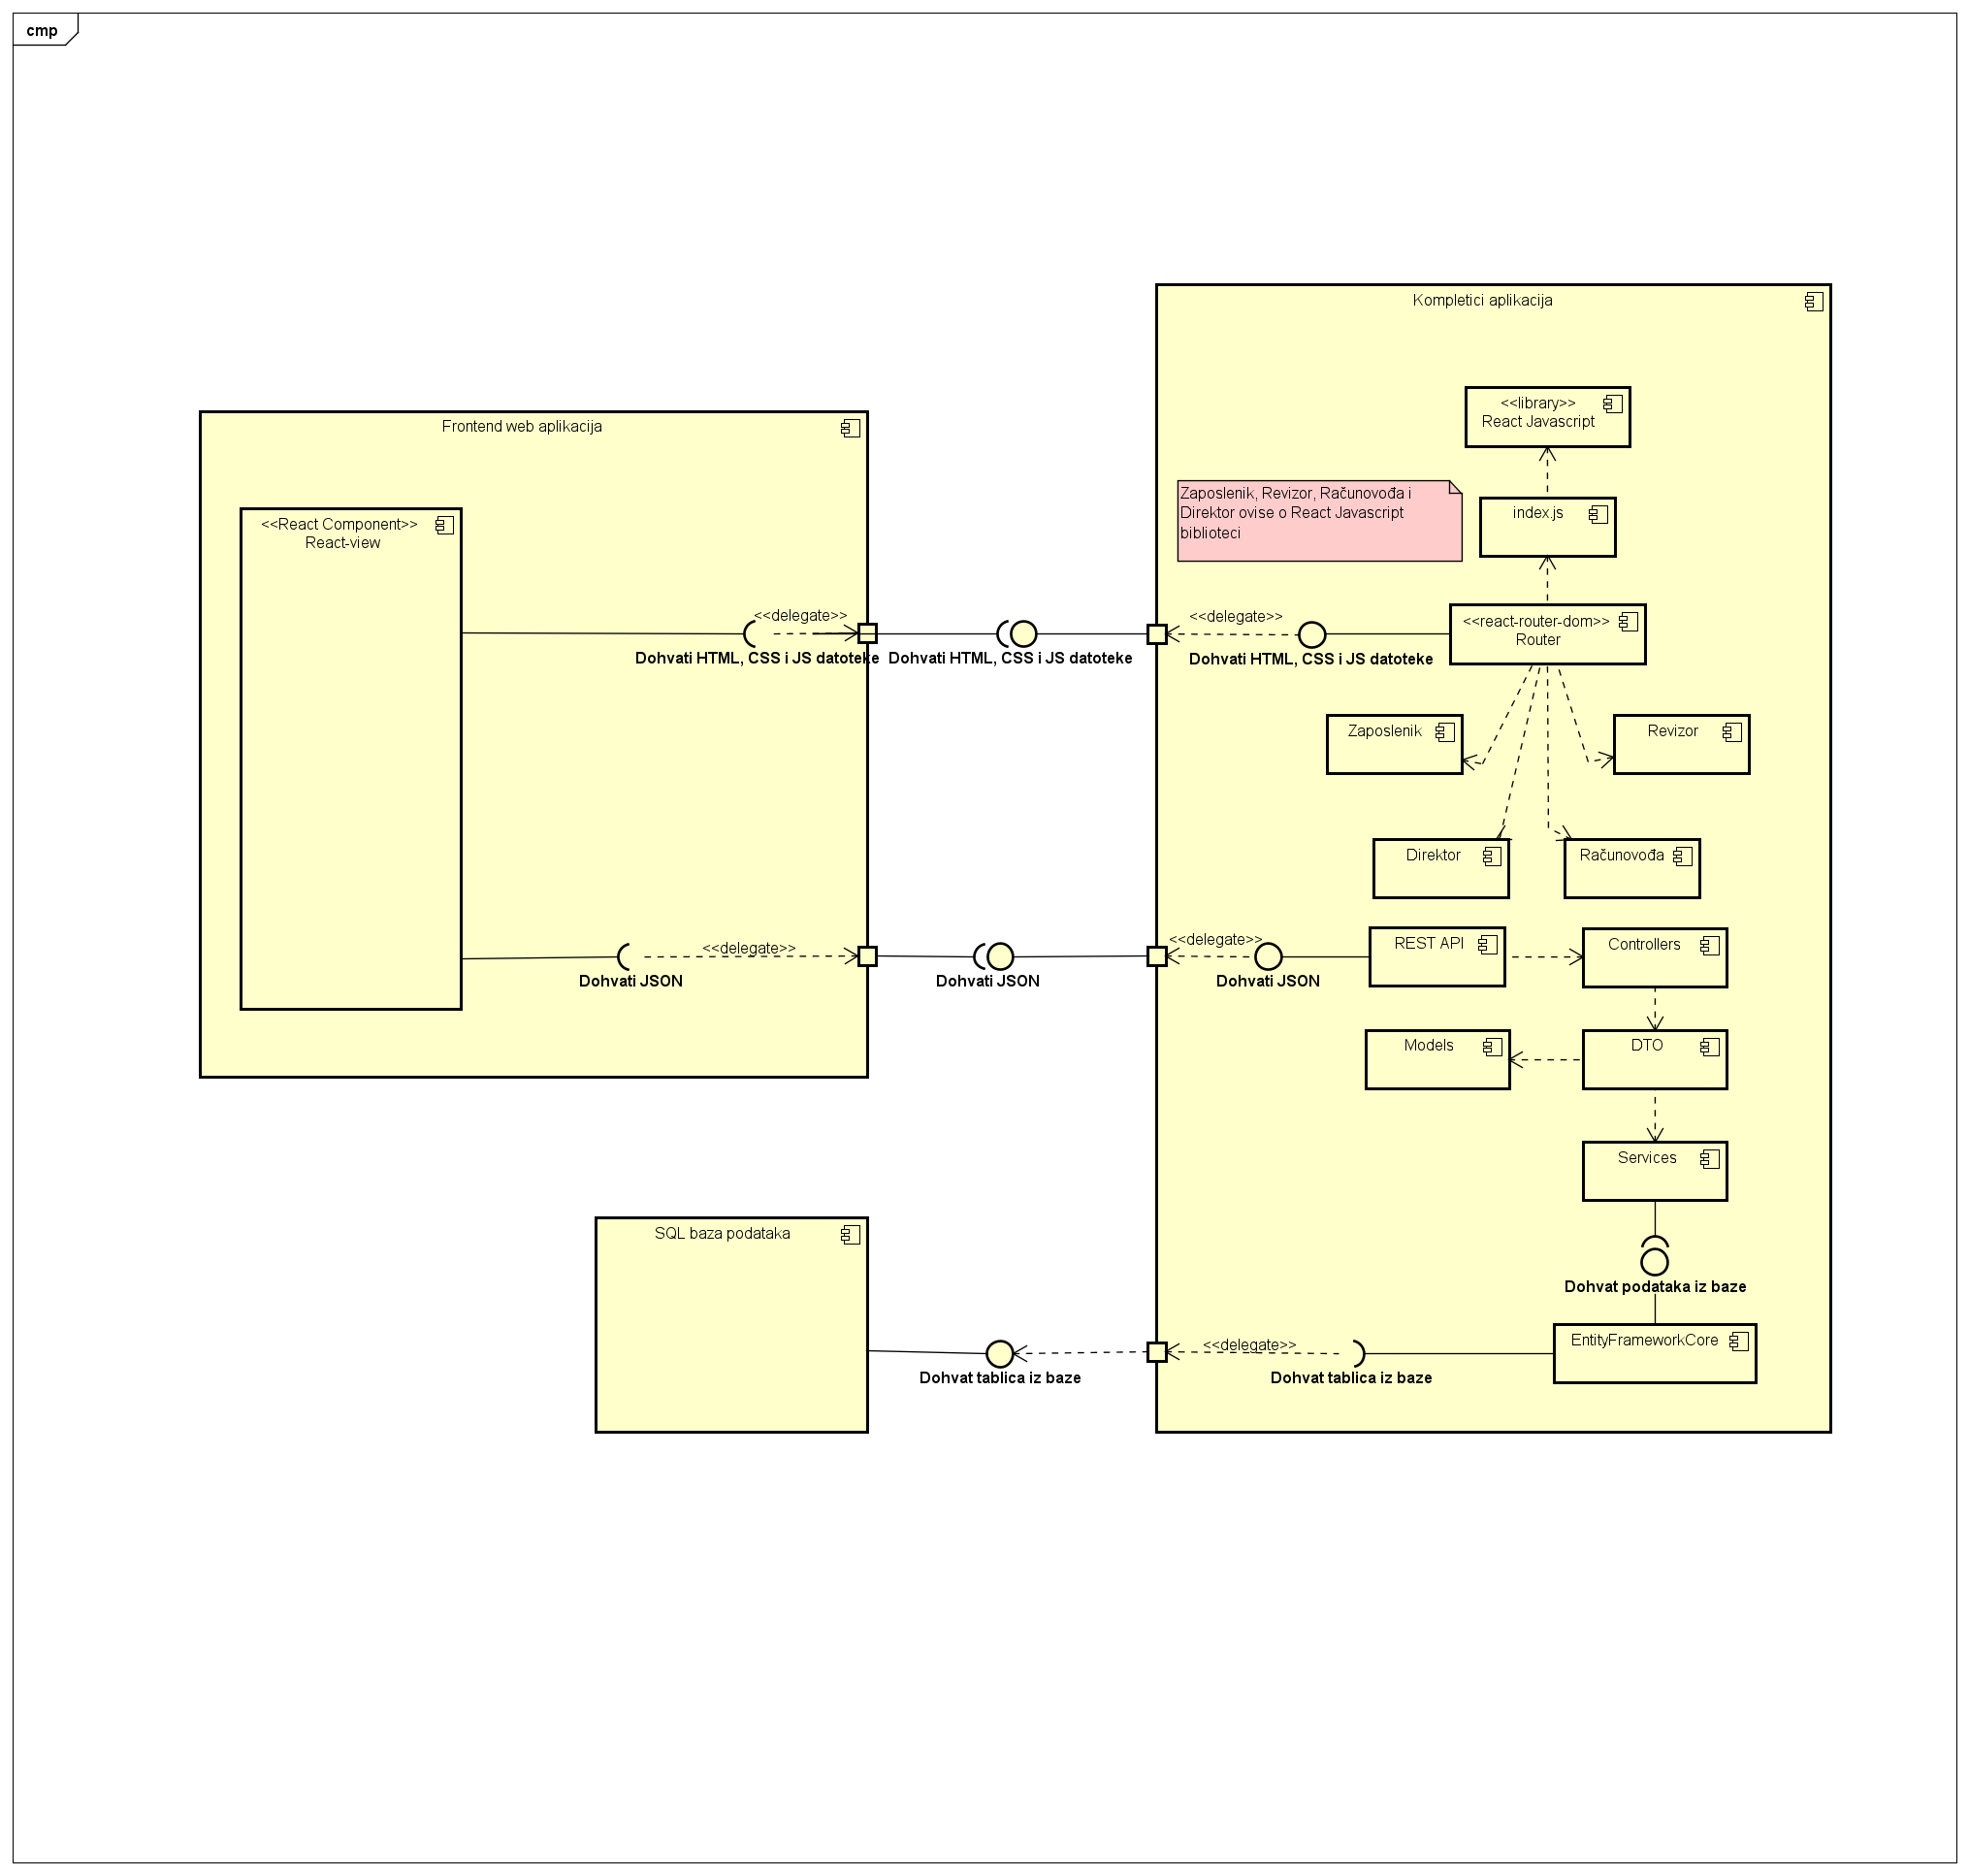
\includegraphics[scale=0.3]{slike/dijagram_komponenti.png} %veličina slike u odnosu na originalnu datoteku i pozicija slike
				\centering
				\caption{Dijagram komponenti}
				\label{fig:promjene}
			\end{figure}
			 
		
		\chapter{Implementacija i korisničko sučelje}
		
		
		\section{Korištene tehnologije i alati}
		
		
			Komunikacija u timu ostvarena je korištenjem aplikacije WhatsApp \footnote{\url{https://www.whatsapp.com/}}. Kao sustav za upravljanje izvornim kodom korišten je Git \footnote{\url{https://git-scm.com/}}, a izvorni kod projekta dostupan je na Github \footnote{\url{https://github.com/}} web platformi . Za izradu dokumentacije korištena je distribucija markup jezika LaTeX MiKTeX \footnote{\url{https://miktex.org/}}  u kombinaciji s TeXstudio \footnote{\url{https://www.texstudio.org/}} radnom okolinom.
				
			Za izradu aplikacije koristila su se dva razvojna okruženja, Visual Studio Code\footnote{\url{https://code.visualstudio.com/}} za frontend i JetBrains IntelliJ IDEA \footnote{\url{https://www.jetbrains.com/idea/}} za backend. Visual Studio Code je radna okolina koju razvija i održava Microsoft, vrlo je fleksibilna te omogućava razvoj u širokom spektru jezika i tehnologija. JetBrains IntelliJ IDEA je razvojno okruženje specifično dizajnirano za rad s programskim jezikom Java, održava je tvrtka JetBrains koja je poznata po proizvodnji razvojnih okolina.
			
			Za izradu backenda korišten je programski jezik Java\footnote{\url{https://www.java.com/en/}} i radni okvir Spring \footnote{\url{https://spring.io/}}. Spring je radni okvir koji nudi gotova rješenja za mnoge često potrebne funkcionalnosti programskih sustava, time programerima omogućuje jednostavniji, brži i sigurniji razvoj aplikacija. 
			
			Za izradu frontenda korišten je programski jezik JavaScript\footnote{\url{https://developer.mozilla.org/en-US/docs/Web/javascript}} i biblioteka React\footnote{\url{https://react.dev/}}. React je biblioteka za razvoj korisničkih sučelja, u složenijim sustavima koristi se s drugim bibliotekama gdje služi kao temeljni sustav sučelja. React održava Facebook.
			
			Za izradu baze podataka korištena je implementacija SQL-a zvana PostgreSQL\footnote{\url{https://www.postgresql.org/}}. 
			
			Za skeniranje dokumenata i njihovo pretvaranje u txt datoteke korišten je OCR Tessaract.\footnote{\url{https://tesseract-ocr.github.io/tessdoc/Home.html}} Tessaract je projekt otvorenog izvornog koda kojeg održava zajednica volontera a omogućuje pretvorbu slika teksta u txt datoteke preko API-a.
			
			Za pohranu slika korištena je Googleova usluga Firebase. Firebase je web platforma za razvoj video igara i aplikacija koja nudi gotova rješenja i infrastrukture. U sklopu ovog projekta korištena je za pohranu slika jer druge usluge nisu dopuštale dovoljno prostora.
			
			Za objavu dokumenata na internetskim mrežama korišten je API društvene mreže Facebook.
			
			Kao platformu za puštanje u pogon odabrane je Render \footnote{\url{https://render.com/}} Render je WEB platforma specifično dizajnirana za puštanje aplikacija u pogon. Render pruža jednostavnu i učinkovitu infrastrukturu u oblaku zajedno s ograničenom memorijom za bazu podataka. Render održava istoimena tvrtka. Kako bi se zadovoljio format u kojem Render očekuje aplikaciju za puštanje u pogon dodatno se koristio alat Docker \footnote{\url{https://www.docker.com/}}. Docker je alat za pakiranje aplikacije sa svim potrebnim sredstvima za pokretanje aplikacije, time se postiže mogućnost pokretanja aplikacije na širokom spektru arhitektura. Docker također održava istoimena tvrtka.
			
		
	
		\section{Ispitivanje programskog rješenja}
			
			\subsection{Ispitivanje komponenti}
			\textit{Potrebno je provesti ispitivanje jedinica (engl. unit testing) nad razredima koji implementiraju temeljne funkcionalnosti. Razraditi \textbf{minimalno 6 ispitnih slučajeva} u kojima će se ispitati redovni slučajevi, rubni uvjeti te izazivanje pogreške (engl. exception throwing). Poželjno je stvoriti i ispitni slučaj koji koristi funkcionalnosti koje nisu implementirane. Potrebno je priložiti izvorni kôd svih ispitnih slučajeva te prikaz rezultata izvođenja ispita u razvojnom okruženju (prolaz/pad ispita). }
			
			
			
			\subsection{Ispitivanje sustava}
			
			Ispitivanje sustava nije provedeno
		
		\section{Dijagram razmještaja}
			
			 Dijagrami razmještaja opisuju topologiju sklopovlja i programsku potporu koja se koristi u implementaciji sustava u njegovom radnom okruženju. Na poslužiteljskom računalu se nalaze web poslužitelj i poslužitelj baze podataka. Klijenti koriste web preglednik kako bi pristupili web aplikaciji. Sustav je baziran na arhitekturi "klijent - poslužitelj", a komunikacija između računala korisnika (zaposlenik, revizor, računovođa, direktor) i poslužitelja odvija se preko HTTP veze.

			 \begin{figure}[H]
				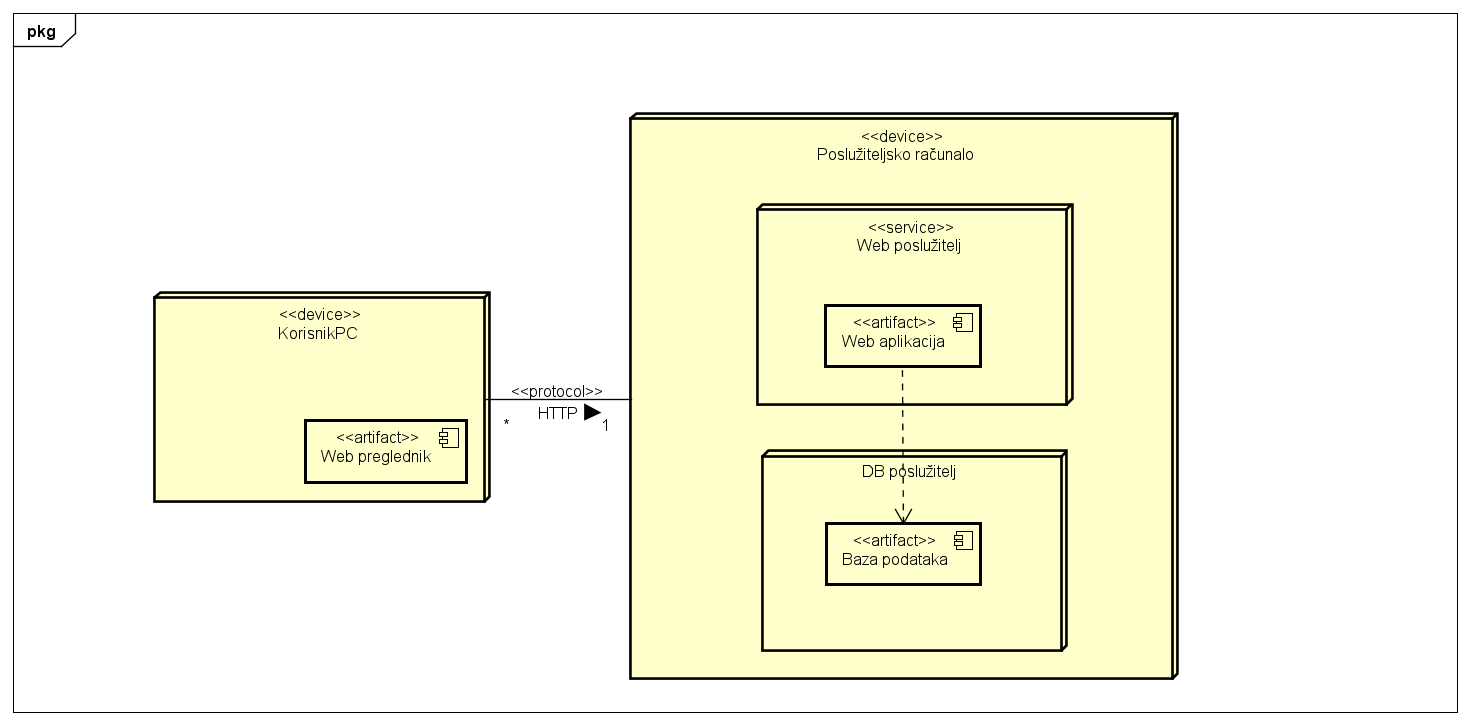
\includegraphics[scale=0.45]{slike/dijagram_razmjestaja.png} %veličina slike u odnosu na originalnu datoteku i pozicija slike
				\centering
				\caption{Dijagram razmještaja}
				\label{fig:promjene}
			\end{figure}
			
			\eject 
		
		\section{Upute za puštanje u pogon}
		
			 
			Za puštanje u pogon korištena je WEB usluga Render istoimene tvrtke, te se puštanje u pogon treba obaviti prema zahtjevima Render platforme. 
			 	
			 \textbf{Konfiguracija poslužitelja baze podataka}
			 
			 Unutar WEB platforme Render potrebno je konfigurirati poslužitelj baze podataka. Na radnoj traci odabiremo opciju new, nakon čega iz padajućeg izbornika treba odabiremo opciju PostgreSQL.
			 
			 
			 \begin{figure}[H]
			 	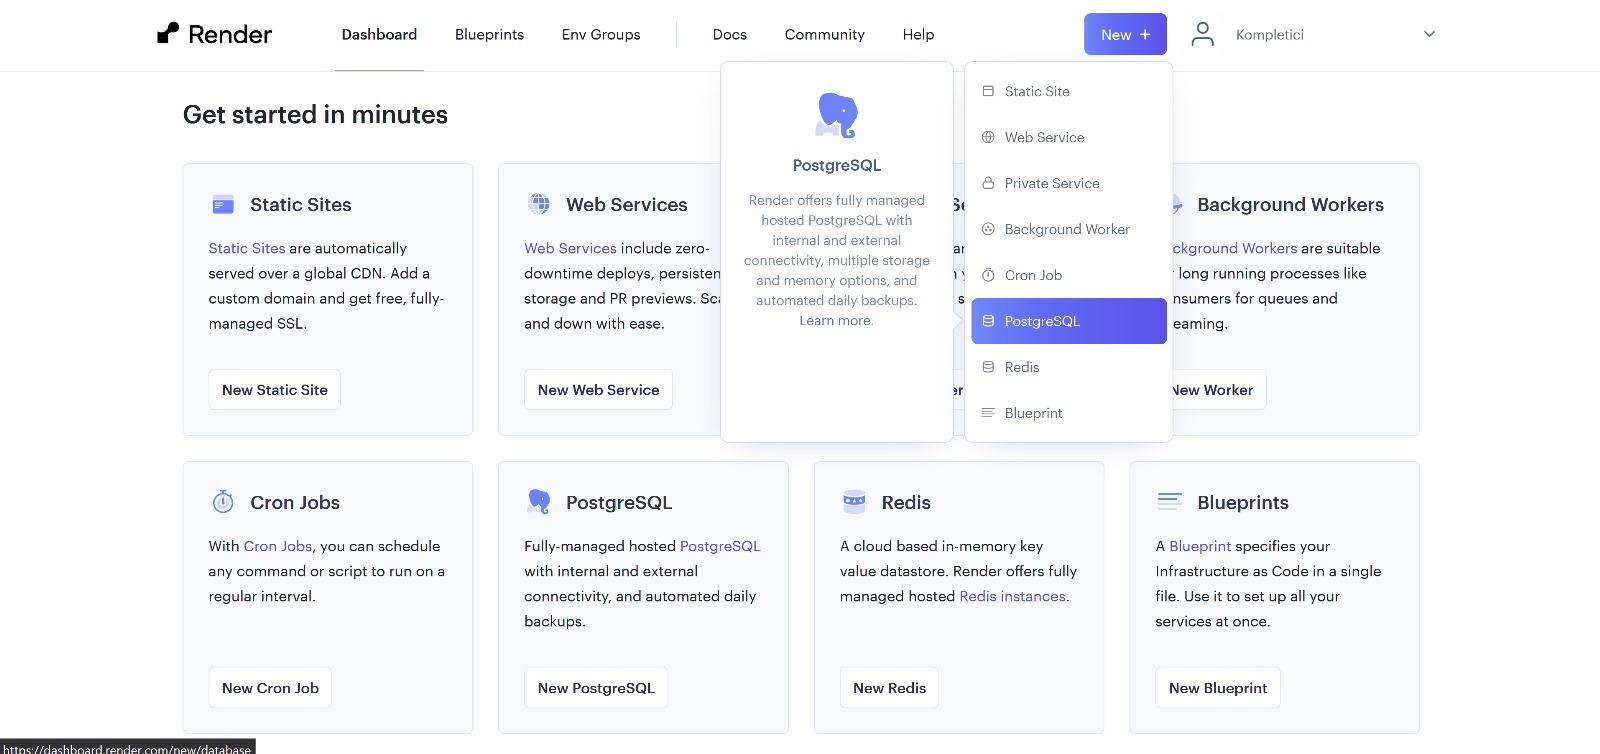
\includegraphics[scale=0.4]{slike/baza_odabir.jpeg} %veličina slike u odnosu na originalnu datoteku i pozicija slike
			 	\centering
			 	\caption{Render korisničko sučelje i radna traka}
			 	\label{fig:promjene}
			 \end{figure}
			 
			 \begin{figure}[H]
			 	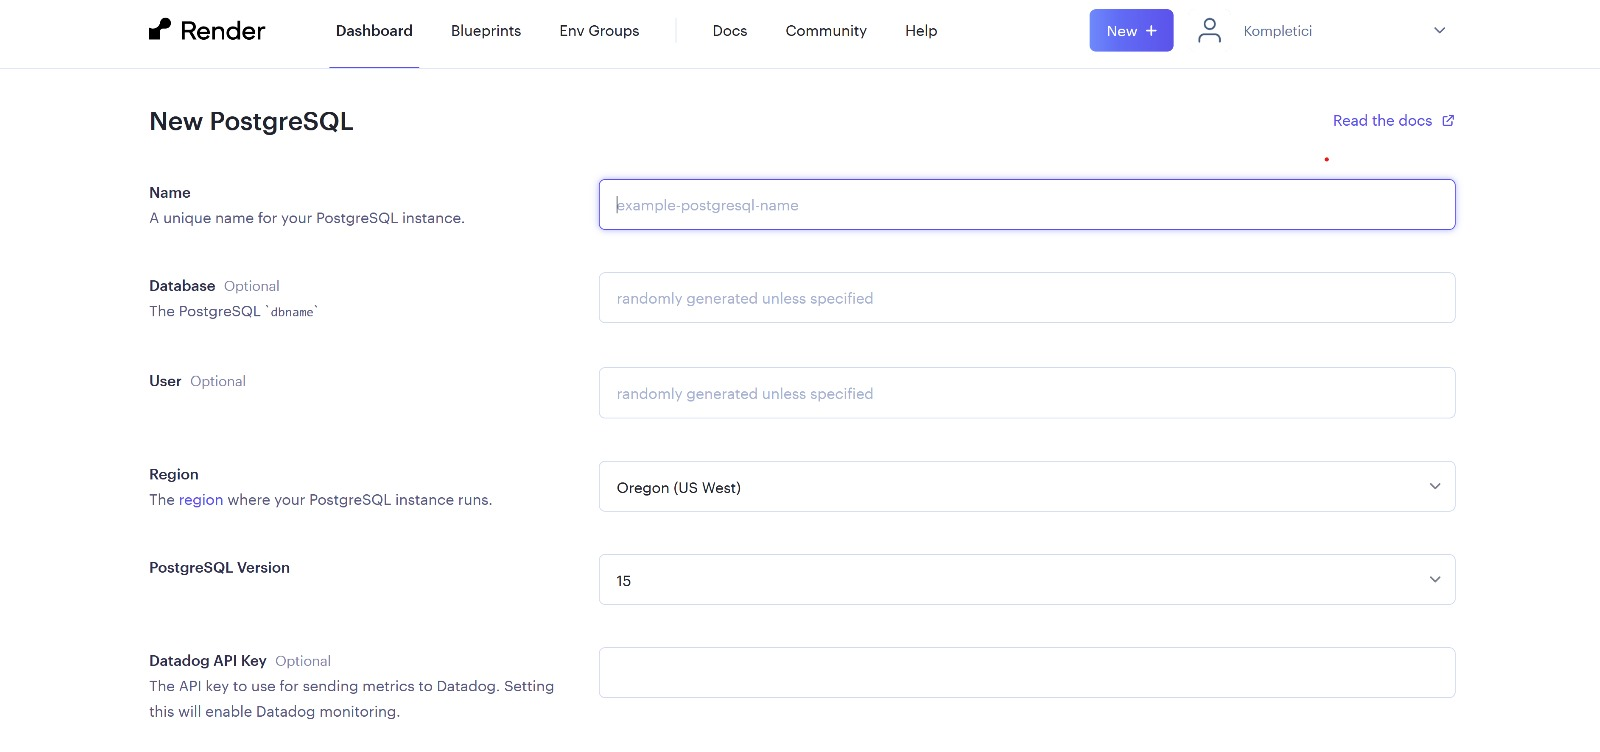
\includegraphics[scale=0.4]{slike/kofiguracija.jpeg} %veličina slike u odnosu na originalnu datoteku i pozicija slike
			 	\centering
			 	\caption{Opcije konfiguracije za bazu podataka}
			 	\label{fig:promjene}
			 \end{figure}
			 
			  Otvoriti će se korisničko sučelje za konfiguraciju baze podataka. Na korisničkom sučelju potrebno je odabrati regiju poslužitelja s kojeg će Render posluživati korisnike. Render će zatim izgenerirati URL poslužitelja baze podataka i lozinku baze podataka, spremamo te podatke jer će nam trebati u daljnjim koracima  

			 \textbf{Konfiguracija backend poslužitelja}
			 
			 Na Render-ovoj radnoj traci odaberemo opciju new WEB service, te odaberemo opciju "Build and deploy from git repository."
			 
			 
			 
			 Nakon toga sljedi proces povezivanja GitHub korisničkog računa i repozitorija s Render korisničkim računom. Potom trebamo odabrati ime za WEB servis te ponovno odabrati regiju poslužitelja s koje će Render posluživati korisnike.
			 
			  \begin{figure}[H]
			 	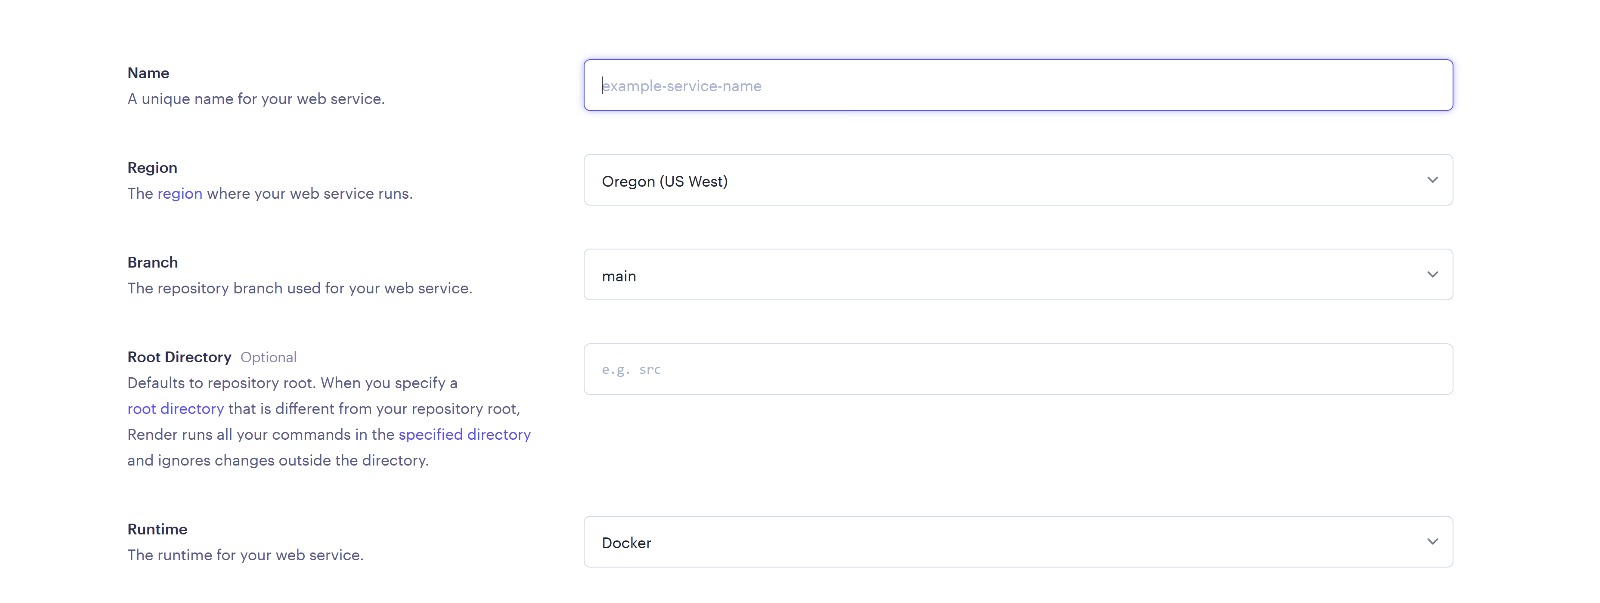
\includegraphics[scale=0.4]{slike/kofiguracija_regije.jpeg} %veličina slike u odnosu na originalnu datoteku i pozicija slike
			 	\centering
			 	\caption{Opcije konfiguracije za WEB servise}
			 	\label{fig:promjene}
			 \end{figure}
			 
			 Nakon toga trebamo odabrati granu GitHub repozitorija s koje će Render povlačiti kod za automatsko puštanje u pogon i odabrati root direktorij backend aplikacije. Za runtime okolinu odabiremo Docker i proširujemo napredne postavke. Dodajemo potrebne varijable okoline poput imena baze, šifre baze i URL baze. Posebnu pozornost trebamo obratiti na format URL-a baze podataka, naime postoji mogućnost da ga treba preoblikovati. On mora biti u sljedećem formatu \textit{\url{jdbc:postgresql://<hostname>:<port>/<database>}}. Konačno moramo dodati putanju Docker datoteke.
			 
			\textbf{Konfiguracija frontend poslužitelja}
			
			
			 Na Renderovoj radnoj traci odabiremo opciju new WEB service, te odabiremo opciju "Build and deploy from git repository." Nakon toga ponovno povezujemo GitHub korisnički račun s Renderom te odabiremo granu koju će Render puštati u pogon. Dodatno odabiremo regiju poslužitelja s kojeg će Render posluživati korisnike. Build komand postavljamo na yarn-build a start komandu na start-prod. Konačno proširujemo napredne postavke te kao varijablu okoline dodajemo adresu deployanog web servisa.
			 
			
			\eject 
		\chapter{Zaključak i budući rad}
		
		
		 
		 	Zadatak projektnog tima bio je razvoj aplikacije za skeniranje i
		 distribuciju dokumenata unutar organizacije. Nakon dva i pol mjeseca rada ostvarili smo zadani cilj. \newline
		 	
			Projekt smo proveli unutar dvije faze razvoja. Prva faza uključivala
		je pisanje početne dokumentacije, odabir tehnologija te podjelu zadataka unutar projektnog tima. Prva faza je također uključivala implementaciju sustava registracije i prijave korisnika te kostur aplikacije. Druga faza sastojala se od implementacije ključnih djelova sustava kao što su skeniranje dokumenata, njihova distribucija i arhiviranje. Dodatno druga faza sadržavala je pisanje popratne dokumentacije.\newline
		 	
		 	Općenito govoreći rad na projektu bio je zanimljivo i korisno iskustvo
		 za sve članove tima. Suočili smo se sa mnogim izazovima od kojih smo mnoge riješili. Glavne prepreke su bile manjak iskustva te ne optimalna koordinacija članova tima. Manjak iskustva stvarao je poteškoće jer su članovi tima morali samostalno učiti tehnologije koje prije nisu koristili te nisu znali najbolje prakse u mnogim situacijama. Ne optimalna koordinacija članova tima značila je da količina posla nije bila u potpunosti ravnopravna te svi članovi tima nisu u potpunosti mogli pridonijeti čak i kad je postojala volja. Poboljšanje radnog procesa u budućim nadogradnjama aplikacije ili radu na novim projektima uključivala bi korištenje poznatih alata i bolju koordinaciju projektnog tima. \newline
		 
		 Implementirali smo sve ključne značajke zadatka. Nedostaje implementacija jednog obrasca uporabe što je mogućnost da direktor mijenja razinu ovlasti drugih korisnika. Neka od poboljšanja koja bi se mogla implementirati su razvoj mobilne aplikacija, poboljšanje robusnosti OCR-a i razvoj boljeg korisničkog sučelja. Iako aplikacija ima mnoge nedostatke zadovoljni smo s odrađenim poslom. 
		 	 
		 	
		
		\eject 
		\chapter*{Popis literature}
		\addcontentsline{toc}{chapter}{Popis literature}
	 	
 		\textbf{\textit{Kontinuirano osvježavanje}}
	
		\textit{Popisati sve reference i literaturu koja je pomogla pri ostvarivanju projekta.}
		
		
		\begin{enumerate}
			
			
			\item  Programsko inženjerstvo, FER ZEMRIS, \url{http://www.fer.hr/predmet/proinz}
			
			\item  I. Sommerville, "Software engineering", 8th ed, Addison Wesley, 2007.
			
			\item  T.C.Lethbridge, R.Langaniere, "Object-Oriented Software Engineering", 2nd ed. McGraw-Hill, 2005.
			
			\item  I. Marsic, Software engineering book``, Department of Electrical and Computer Engineering, Rutgers University, \url{http://www.ece.rutgers.edu/~marsic/books/SE}
			
			\item  The Unified Modeling Language, \url{https://www.uml-diagrams.org/}
			
			\item  Astah Community, \url{http://astah.net/editions/uml-new}
		\end{enumerate}
		
		 
		
		
		\begingroup
		\renewcommand*\listfigurename{Indeks slika i dijagrama}
		%\renewcommand*\listtablename{Indeks tablica}
		%\let\clearpage\relax
		\listoffigures
		%\vspace{10mm}
		%\listoftables
		\endgroup
		\addcontentsline{toc}{chapter}{Indeks slika i dijagrama}
		
		
		
		\eject 
		
		%\chapter*{Dodatak: Prikaz aktivnosti grupe}
		\addcontentsline{toc}{chapter}{Dodatak: Prikaz aktivnosti grupe}
		
		\section*{Dnevnik sastajanja}
		
		\textbf{\textit{Kontinuirano osvježavanje}}\\
		
		 \textit{U ovom dijelu potrebno je redovito osvježavati dnevnik sastajanja prema predlošku.}
		
		\begin{packed_enum}
			\item  sastanak
			
			\item[] \begin{packed_item}
				\item Datum: u ovom formatu: \today
				\item Prisustvovali: I.Prezime, I.Prezime
				\item Teme sastanka:
				\begin{packed_item}
					\item  opis prve teme
					\item  opis druge teme
				\end{packed_item}
			\end{packed_item}
			
			\item  sastanak
			\item[] \begin{packed_item}
				\item Datum: u ovom formatu: \today
				\item Prisustvovali: I.Prezime, I.Prezime
				\item Teme sastanka:
				\begin{packed_item}
					\item  opis prve teme
					\item  opis druge teme
				\end{packed_item}
			\end{packed_item}
			
			%
			
		\end{packed_enum}
		
		\eject
		\section*{Tablica aktivnosti}
		
			\textbf{\textit{Kontinuirano osvježavanje}}\\
			
			 \textit{Napomena: Doprinose u aktivnostima treba navesti u satima po članovima grupe po aktivnosti.}

			\begin{longtblr}[
					label=none,
				]{
					vlines,hlines,
					width = \textwidth,
					colspec={X[7, l]X[1, c]X[1, c]X[1, c]X[1, c]X[1, c]X[1, c]X[1, c]}, 
					vline{1} = {1}{text=\clap{}},
					hline{1} = {1}{text=\clap{}},
					rowhead = 1,
				} 
			
				\SetCell[c=1]{c}{} & \SetCell[c=1]{c}{\rotatebox{90}{\textbf{Ime Prezime voditelja}}} & \SetCell[c=1]{c}{\rotatebox{90}{\textbf{Ime Prezime }}} &	\SetCell[c=1]{c}{\rotatebox{90}{\textbf{Ime Prezime }}} & \SetCell[c=1]{c}{\rotatebox{90}{\textbf{Ime Prezime }}} &	\SetCell[c=1]{c}{\rotatebox{90}{\textbf{Ime Prezime }}} & \SetCell[c=1]{c}{\rotatebox{90}{\textbf{Ime Prezime }}} &	\SetCell[c=1]{c}{\rotatebox{90}{\textbf{Ime Prezime }}} \\  
				Upravljanje projektom 		&  &  &  &  &  &  & \\ 
				Opis projektnog zadatka 	&  &  &  &  &  &  & \\ 
				
				Funkcionalni zahtjevi       &  &  &  &  &  &  &  \\ 
				Opis pojedinih obrazaca 	&  &  &  &  &  &  &  \\ 
				Dijagram obrazaca 			&  &  &  &  &  &  &  \\ 
				Sekvencijski dijagrami 		&  &  &  &  &  &  &  \\ 
				Opis ostalih zahtjeva 		&  &  &  &  &  &  &  \\ 

				Arhitektura i dizajn sustava	 &  &  &  &  &  &  &  \\ 
				Baza podataka				&  &  &  &  &  &  &   \\ 
				Dijagram razreda 			&  &  &  &  &  &  &   \\ 
				Dijagram stanja				&  &  &  &  &  &  &  \\ 
				Dijagram aktivnosti 		&  &  &  &  &  &  &  \\ 
				Dijagram komponenti			&  &  &  &  &  &  &  \\ 
				Korištene tehnologije i alati 		&  &  &  &  &  &  &  \\ 
				Ispitivanje programskog rješenja 	&  &  &  &  &  &  &  \\ 
				Dijagram razmještaja			&  &  &  &  &  &  &  \\ 
				Upute za puštanje u pogon 		&  &  &  &  &  &  &  \\  
				Dnevnik sastajanja 			&  &  &  &  &  &  &  \\ 
				Zaključak i budući rad 		&  &  &  &  &  &  &  \\  
				Popis literature 			&  &  &  &  &  &  &  \\  
				&  &  &  &  &  &  &  \\ \hline 
				\textit{Dodatne stavke kako ste podijelili izradu aplikacije} 			&  &  &  &  &  &  &  \\ 
				\textit{npr. izrada početne stranice} 				&  &  &  &  &  &  &  \\  
				\textit{izrada baze podataka} 		 			&  &  &  &  &  &  & \\  
				\textit{spajanje s bazom podataka} 							&  &  &  &  &  &  &  \\ 
				\textit{back end} 							&  &  &  &  &  &  &  \\  
				 							&  &  &  &  &  &  &\\ 
			\end{longtblr}
					
					
		\eject
		\section*{Dijagrami pregleda promjena}
		
		\textbf{\textit{dio 2. revizije}}\\
		
		\textit{Prenijeti dijagram pregleda promjena nad datotekama projekta. Potrebno je na kraju projekta generirane grafove s gitlaba prenijeti u ovo poglavlje dokumentacije. Dijagrami za vlastiti projekt se mogu preuzeti s gitlab.com stranice, u izborniku Repository, pritiskom na stavku Contributors.}
		
	
		
		
	\end{document} %naredbe i tekst nakon ove naredbe ne ulaze u izgrađen dokument 